%% =====================================================================
%% Operator-Adaptive Kernel Ridge Regression for Near-Infrared Spectroscopy
%% Companion paper to the AOM-PLS manuscript
%% Manuscript class: \documentclass{article} as requested by the brief.
%% (The AOM-PLS companion uses Elsevier elsarticle; we adopt the
%% standard `article` class here at the brief's request, while keeping
%% the same package list, macros, and section conventions.)
%% =====================================================================

\documentclass[11pt,a4paper]{article}

%% --- Packages -------------------------------------------------------
\usepackage[utf8]{inputenc}
\usepackage[T1]{fontenc}
\usepackage{amsmath,amssymb}
\usepackage{mathtools}
\usepackage{bm}
\usepackage{booktabs}
\usepackage{graphicx}
\graphicspath{{../figures/}}
%% for missing figure files; remove the option once figures are available.
\usepackage{xcolor}
\usepackage{hyperref}
\usepackage{url}
\usepackage{lmodern}
\usepackage{microtype}
\usepackage{enumitem}
\usepackage{caption}
\usepackage{natbib}
\usepackage{xspace}
\usepackage{geometry}
\geometry{margin=2.5cm}

\hypersetup{
  colorlinks=true,
  linkcolor=blue!50!black,
  citecolor=blue!50!black,
  urlcolor=blue!50!black,
}

%% --- Macros ---------------------------------------------------------
\newcommand{\R}{\mathbb{R}}
\newcommand{\identity}{\mathbf{I}}
\newcommand{\Xmat}{\mathbf{X}}
\newcommand{\Ymat}{\mathbf{Y}}
\newcommand{\Yc}{\mathbf{Y}_{\!c}}
\newcommand{\Amat}{\mathbf{A}}
\newcommand{\Smat}{\mathbf{S}}
\newcommand{\Zmat}{\mathbf{Z}}
\newcommand{\Kmat}{\mathbf{K}}
\newcommand{\Umat}{\mathbf{U}}
\newcommand{\Mmat}{\mathbf{M}}
\newcommand{\Cmat}{\mathbf{C}}
\newcommand{\Rmat}{\mathbf{R}}
\newcommand{\Tmat}{\mathbf{T}}
\newcommand{\Imat}{\mathbf{I}}
\newcommand{\tvec}{\mathbf{t}}
\newcommand{\Phimat}{\mathbf{\Phi}}
\newcommand{\xvec}{\mathbf{x}}
\newcommand{\yvec}{\mathbf{y}}
\newcommand{\PLS}{\textsc{PLS}\xspace}
\newcommand{\AOM}{\textsc{AOM}\xspace}
\newcommand{\AOMR}{\textsc{AOM-Ridge}\xspace}
\newcommand{\SNV}{\textsc{SNV}\xspace}
\newcommand{\MSC}{\textsc{MSC}\xspace}
\newcommand{\EMSC}{\textsc{EMSC}\xspace}
\newcommand{\AsLS}{\textsc{AsLS}\xspace}
\newcommand{\nirsfourall}{\texttt{nirs4all}\xspace}

\title{Operator-Adaptive Kernel Ridge Regression for\\
Near-Infrared Spectroscopy: Dual Formulation, Branch-CV, and MKL-Light}

\author{Gr\'egory Beurier\\
\texttt{gregory.beurier@cirad.fr}\\
\nirsfourall open-source project, France}

\date{}

\begin{document}

\maketitle

%% =====================================================================
%% Abstract for "AOM-Ridge: Operator-Adaptive Kernel Ridge Regression
%% for Near-Infrared Spectroscopy"
%% =====================================================================

\begin{abstract}
Ridge regression is a strong baseline for near-infrared spectroscopy
(NIRS) calibration but, like \PLS, it depends on a long chain of
spectral preprocessing decisions that practitioners typically search as
an external Cartesian grid. We present \emph{Operator-Adaptive Kernel
Ridge Regression} (\AOMR), a kernel formulation that absorbs that
preprocessing search into the Ridge solve itself. Each strict linear
spectral operator $\Amat_b\in\R^{p\times p}$ defines a view
$\Xmat_b=\Xmat\Amat_b^\top$; we form the superblock dual kernel
$K=\sum_b s_b^2\,\Xmat\Amat_b^\top\Amat_b\Xmat^\top$ and a metric matrix
$U=\sum_b s_b^2\Amat_b^\top\Amat_b\Xmat^\top$ such that the original-
space Ridge coefficient is $\bm\beta=U C$ with
$C=(K+\alpha I)^{-1}\Yc$. Because Ridge is geometry-dependent, the
covariance-space shortcut available to \PLS does not extend to Ridge:
the kernel must be assembled explicitly per operator. The estimator
exposes five selection modes --- \texttt{superblock} (one Ridge over the
full bank), \texttt{global} (hard $(b^\star,\alpha^\star)$ selection by
fold-local CV), \texttt{active\_superblock} (top-$m$ + diversity
pruning), \texttt{branch\_global} (fold-local CV over (branch, op,
$\alpha$) with non-strict-linear branches), and \texttt{mkl}
(kernel-target-alignment weighted block sum) --- all of which run on
top of a single fold-local CV core that rebuilds means, operator
clones, scales, and kernels inside every fold. We further introduce
six methodological extensions (a ten-branch \texttt{branch\_global}
covering the full SNV/MSC/EMSC/AsLS family, a split-aware inner CV for
$y$-based stress splits, a soft multi-branch MKL, a local Ridge in
score space, and convex blender / auto-selector aggregators) and
companion \emph{AOM-Ridge-PLS} that ridge-regresses on PLS rotations of
the operator-mixture superblock. Anti-leakage is verified by spy
operators that fail when any fold-local invariant is broken. On a
54-dataset NIRS regression cohort assembled from the TabPFN paper
benchmark, the strongest single deployable variant
(\texttt{Blender}, a convex non-negative blend of out-of-fold
predictions over an 8-candidate pool) wins on $\bm{35/52}$
datasets ($67.3\%$) against the published Ridge HPO baseline with
median test-RMSEP delta of $\bm{-2.22\%}$, beats PLS on $79\%$ and
TabPFN-Raw on $57\%$, but loses to TabPFN-opt at $38\%$ wins
(median $+4.72\%$). Beyond a single deployable variant, the
\emph{oracle envelope} (best of $V=29$ benched variants per
dataset, an upper bound that requires test-set knowledge and is
not directly deployable) wins on $\bm{45/52}$ datasets ($86.5\%$)
against Ridge HPO (median $-4.73\%$) and \emph{ties} TabPFN-opt at
$51.9\%$ wins (median $-0.21\%$); the $\sim 2.5$\,pp oracle
--blender gap is the headroom left for a smarter meta-selector.
The estimator returns an original-space coefficient
$\bm\beta\in\R^{p\times q}$, is sklearn-compatible, and is shipped as a
self-contained package (\texttt{aomridge}) under
\texttt{bench/AOM\_v0/Ridge/}.
\end{abstract}

\medskip
\noindent\textbf{Keywords:} Ridge regression; kernel methods; NIRS;
operator-adaptive preprocessing; multiple kernel learning; TabPFN;
reproducible benchmark.


%% =====================================================================
\section{Introduction}\label{sec:intro}
%% =====================================================================

Near-infrared spectroscopy (NIRS) calibration is a high-dimensional,
small-$n$ regression problem~\citep{williams2007implementation,
rinnan2009review}. Spectra contain hundreds to thousands of strongly
correlated channels, and most public NIRS datasets contain only a few
hundred labelled samples. In this regime Ridge
regression~\citep{hoerl1970ridge, hoerl1970application,
hastie2009elements} is a strong baseline: the $\ell_2$ penalty
controls the variance inflation that ordinary least squares would
suffer from, and the closed-form solution makes it cheap to evaluate
many regularisation strengths $\alpha$ via a single eigendecomposition
of the kernel $\Kmat=\Xmat\Xmat^\top$~\citep{saunders1998ridge,
scholkopf2002learning}. The reference results published with the
TabPFN tabular foundation model paper~\citep{hollmann2023tabpfn,
hollmann2025tabpfn} use Ridge as one of the four classical baselines on
their NIRS regression cohort, after a non-trivial preprocessing search
(\SNV, \MSC, Savitzky-Golay smoothing/derivatives, detrend, baseline
correction) and an Optuna-driven $\alpha$ tuning. We refer to this
configuration in the rest of the paper as \emph{paper Ridge HPO}.

The cost of paper Ridge HPO is the cost of \emph{any} preprocessing
grid search: the analyst picks a finite Cartesian product of operator
choices, runs Ridge on each, and reports the best one against an
external split. Two analysts with the same data and the same operator
inventory can reach different pipelines, the runs are not auditable,
and the search is irreproducible across software stacks because the
Cartesian product itself is implementation-defined. The companion
paper for AOM-PLS~\citep{beurier2026aompls} addresses the same problem
for \PLS by absorbing the preprocessing search into the latent
extraction loop: every strict linear spectral operator
$\Amat\in\R^{p\times p}$ acts as $\Xmat\Amat^\top$ on row spectra,
and the cross-covariance identity
$(\Xmat\Amat^\top)^\top\Ymat=\Amat\Xmat^\top\Ymat$ lets one evaluate
operator candidates in covariance space without ever materialising the
transformed matrix. The AOM-PLS companion paper is parity-validated
against the deployed \nirsfourall \texttt{AOMPLSRegressor} and reports
median improvements over \PLS on the TabPFN/NIRS cohort.

This paper asks the same methodological question for Ridge: \emph{can
a bank of strict linear preprocessing operators be absorbed into the
Ridge solve itself?} The answer requires more care than for \PLS.
Ridge is a \emph{geometry}-dependent estimator: the loss
$\|\Ymat-\Xmat\bm\beta\|_F^2+\alpha\|\bm\beta\|_F^2$ depends on the
inner product of $\Xmat$, not just on its cross-covariance with
$\Ymat$. The covariance-space shortcut at the heart of AOM-PLS is
therefore not available to AOM-Ridge: every operator changes the
kernel, and the kernel is what the Ridge solve actually sees. The
AOM-Ridge formulation is therefore a kernel formulation in the strict
sense. We form a single dual kernel
$\Kmat=\sum_b s_b^2\,\Xmat\Amat_b^\top\Amat_b\Xmat^\top$ over a bank
of strict-linear operators, solve the dual Ridge problem
$(\Kmat+\alpha\identity)\Cmat=\Yc$ once, and recover the original-
space coefficient $\bm\beta\in\R^{p\times q}$ via a metric matrix
$\Umat=\sum_b s_b^2\Amat_b^\top\Amat_b\Xmat^\top$.

The contributions of this work are:
\begin{enumerate}[leftmargin=2em,label=(\arabic*)]
  \item a \textbf{dual / kernel AOM-Ridge formulation}
        (Sections~\ref{sec:method-single}--\ref{sec:method-superblock})
        with an original-space coefficient $\bm\beta=\Umat\Cmat$ that
        makes the estimator a drop-in replacement for
        \texttt{sklearn.linear\_model.Ridge};
  \item a \textbf{family of selection modes}
        (Section~\ref{sec:method-selection}): \texttt{superblock} (one
        Ridge over the union of views), \texttt{global} (hard
        $(b^\star,\alpha^\star)$ selection by fold-local CV),
        \texttt{active\_superblock} (top-$m$ + diversity pruning),
        \texttt{branch\_global} (fold-local CV over (branch, op,
        $\alpha$) where branches in
        \{\texttt{none},\SNV,\MSC\} carry non-strict-linear
        preprocessing), and \texttt{mkl} (kernel-target-alignment
        weighted block sum);
  \item a \textbf{fold-local CV core}
        (Section~\ref{sec:method-foldlocal}) with documented
        anti-leakage invariants and spy-operator regression tests that
        fail when the invariants are broken;
  \item an \textbf{adaptive alpha grid} with boundary-expansion
        (Section~\ref{sec:method-alpha}) and a one-standard-error
        selection rule, which together remove most of the residual
        sensitivity to the user-supplied alpha range;
  \item a \textbf{39-dataset NIRS regression benchmark}
        (Sections~\ref{sec:experiments}--\ref{sec:results}) on the
        TabPFN paper cohort against six baselines (Ridge, \PLS, CNN,
        CatBoost, TabPFN-Raw, TabPFN-opt) and an explicit comparison
        against published \emph{paper Ridge HPO} results.
\end{enumerate}

The headline result is that \AOMR\ wins on \textbf{32/38 datasets
(84\%)} against paper Ridge HPO, with a median test-RMSEP delta of
\textbf{$-4.94\%$}. The \texttt{global} mode contributes the largest
share of dataset wins ($\sim$33\%), followed by the SNV-branch variant
of \texttt{global} ($\sim$26\%) and the family-pruned SNV variant
($\sim$15\%). Limitations and failure modes are discussed in
Section~\ref{sec:discussion}: AMYLOSE-style $y$-based splits where
inner CV is not predictive of test performance, and outlier datasets
(BEER \texttt{YbaseSplit}, TIC) where SNV is selected by inner CV but
raw spectra would be the better choice. We do not claim that
\AOMR\ beats TabPFN-opt with its per-dataset hyperparameter
optimisation~\citep{hollmann2025tabpfn}; we claim a parity-grade
Ridge baseline that absorbs the preprocessing search.

\paragraph{Relation to AOM-PLS.}
\AOMR\ is the companion of AOM-PLS~\citep{beurier2026aompls} for the
Ridge family. The two estimators share the operator bank
infrastructure (\texttt{aompls.banks}, \texttt{aompls.operators}) but
otherwise reach the operator-adaptive goal through different routes:
AOM-PLS exploits the cross-covariance identity to evaluate operators
without materialising $\Xmat\Amat^\top$, while AOM-Ridge must assemble
the kernel explicitly because the Ridge geometry depends on
$\Xmat\Amat^\top\Amat\Xmat^\top$, not on $\Amat\Xmat^\top\Ymat$. The
two papers can be read independently.

%% =====================================================================
\section{Method}\label{sec:method}
%% =====================================================================

\subsection{Notation and the strict-linear operator contract}\label{sec:method-notation}

Let $\Xmat\in\R^{n\times p}$ collect $n$ row spectra of length $p$ and
$\Ymat\in\R^{n\times q}$ the response matrix ($q=1$ for univariate
regression). A \emph{strict linear spectral operator} is a matrix
$\Amat\in\R^{p\times p}$ that acts on row spectra by right-
multiplication of its transpose:
\begin{equation}
\Xmat_b \;=\; \Xmat\,\Amat_b^\top.
\label{eq:operator-action}
\end{equation}
A \emph{bank} is a finite set
$\mathcal{B}=\{\Amat_1,\dots,\Amat_B\}$ where $\Amat_1$ is the identity
(prepended automatically; duplicate identities are deduplicated). The
banks supported by \AOMR\ are imported from the AOM-PLS package and
include \texttt{compact} ($|\mathcal{B}|=9$), \texttt{default}
($|\mathcal{B}|=100$), \texttt{family\_pruned} ($|\mathcal{B}|=15$, one
representative per family), \texttt{response\_dedup} ($|\mathcal{B}|=46$,
response-cosine pruned), and the deeper \texttt{deep3} / \texttt{deep4}
research banks. \emph{Strict linearity} is essential: SNV and MSC have
row-dependent parameters, so they are not strict-linear operators in
this sense; they appear in \AOMR\ only as \emph{branch} preprocessors,
covered in Section~\ref{sec:method-selection}.

Centering. All formulations below apply Ridge in centered form. Let
$\bar{\xvec}=\Xmat^\top\bm 1/n$ and
$\bar{\yvec}=\Ymat^\top\bm 1/n$ be training-fold means; we write
$\Xmat_c=\Xmat-\bar{\xvec}^\top$ and $\Yc=\Ymat-\bar{\yvec}^\top$.
Predictions on a new spectrum $\xvec_\star$ are
$\hat{\yvec}_\star=(\xvec_\star-\bar{\xvec})^\top\bm\beta+\bar{\yvec}$.
With $\bm\beta\in\R^{p\times q}$ the original-space coefficient, the
intercept absorbs the centering: $\hat{\Ymat}=\Xmat\bm\beta+\bm c$
with $\bm c=\bar{\yvec}-\bar{\xvec}^\top\bm\beta$.

\subsection{Single-operator dual Ridge}\label{sec:method-single}

For one strict linear operator $\Amat_b$, define
$\Zmat_b=\Xmat_c\Amat_b^\top$. The Ridge problem in the transformed
space is
\begin{equation}
\min_{\bm\gamma}\;\|\Yc-\Zmat_b\bm\gamma\|_F^2 + \alpha\|\bm\gamma\|_F^2,
\end{equation}
with closed-form primal solution
$\bm\gamma_b=(\Zmat_b^\top\Zmat_b+\alpha\identity_p)^{-1}\Zmat_b^\top\Yc$.
For high-dimensional NIRS spectra ($p\gg n$) the dual form is much
cheaper. Define
\begin{align}
\Kmat_b &\;=\; \Zmat_b\Zmat_b^\top
            \;=\; \Xmat_c\Amat_b^\top\Amat_b\Xmat_c^\top, \\
\Cmat_b &\;=\; (\Kmat_b+\alpha\identity_n)^{-1}\Yc, \\
\bm\beta_b &\;=\; \Amat_b^\top\Amat_b\Xmat_c^\top\Cmat_b.
\label{eq:single-beta}
\end{align}
The original-space coefficient $\bm\beta_b\in\R^{p\times q}$ is a key
deliverable: it makes the estimator a drop-in replacement for
\texttt{sklearn.linear\_model.Ridge}, and it lets the estimator predict
on raw $\Xmat$ without remembering the operator at all (provided one
keeps $\bar{\xvec}$ and $\bar{\yvec}$). Predictions can be computed
either in primal form $\hat{\Ymat}_c=\Xmat_{*c}\bm\beta_b$ or in dual
form $\hat{\Ymat}_c=\Kmat_{*b}\Cmat_b$ with
$\Kmat_{*b}=\Xmat_{*c}\Amat_b^\top\Amat_b\Xmat_c^\top$; both must be
numerically identical and are tested for equality in the unit suite.

\subsection{Superblock dual Ridge}\label{sec:method-superblock}

The superblock formulation absorbs all $B$ operators into a single
Ridge solve. Define the wide concatenated matrix
\begin{equation}
\Phimat(\Xmat_c) \;=\; \big[\,s_1\Xmat_c\Amat_1^\top \;\big|\; s_2\Xmat_c\Amat_2^\top \;\big|\;\cdots\;\big|\; s_B\Xmat_c\Amat_B^\top\,\big]
\;\in\;\R^{n\times Bp},
\label{eq:phi-superblock}
\end{equation}
where $s_b>0$ are per-block scales (Section~\ref{sec:method-blockscale}).
The wide-form Ridge problem
\begin{equation}
\min_{\bm\gamma\in\R^{Bp\times q}}\;\|\Yc-\Phimat\bm\gamma\|_F^2 + \alpha\|\bm\gamma\|_F^2
\end{equation}
has the dual kernel
\begin{equation}
\Kmat \;=\; \Phimat\Phimat^\top \;=\; \sum_{b=1}^B s_b^2\,\Xmat_c\Amat_b^\top\Amat_b\Xmat_c^\top.
\label{eq:superblock-kernel}
\end{equation}
The crucial observation for the AOM-Ridge implementation is that we
\emph{never} materialise $\Phimat$ (which would have $Bp$ columns).
Define the metric matrix
\begin{equation}
\Mmat \;=\; \sum_{b=1}^B s_b^2\,\Amat_b^\top\Amat_b \;\in\;\R^{p\times p},
\qquad
\Umat \;=\; \Mmat\Xmat_c^\top \;\in\;\R^{p\times n},
\qquad
\Kmat \;=\; \Xmat_c\Umat.
\label{eq:M-U-K}
\end{equation}
The dual coefficients and the original-space regression coefficient
follow:
\begin{equation}
\Cmat \;=\; (\Kmat+\alpha\identity_n)^{-1}\Yc,
\qquad
\bm\beta \;=\; \Umat\Cmat \;=\; \Mmat\Xmat_c^\top\Cmat.
\label{eq:beta-superblock}
\end{equation}
The estimator exposes \texttt{coef\_=}$\bm\beta$ with shape $(p,q)$,
\emph{never} a wide $(Bp,q)$ coefficient. This is enforced by a
shape-assertion test in the unit suite. In implementation,
$\Umat$ is built one operator at a time:
$\Umat=\sum_b s_b^2\,\Amat_b^\top(\Amat_b\Xmat_c^\top)$, so the cost
is $\mathcal{O}(B\,np)$ kernel-application time when each $\Amat_b$ is
banded (the typical case for SG/detrend/finite-difference operators).

\paragraph{Equivalence with the explicit superblock.}
The unit suite verifies that the dual kernel of
Equation~\eqref{eq:superblock-kernel} produces the same predictions
and the same $\bm\beta$ as the explicitly concatenated $\Phimat$
followed by sklearn \texttt{Ridge}, up to floating-point tolerance.
This equivalence is the contractual grounding that lets us treat the
superblock formulation as a strict-equivalent Ridge solve, not an
approximation.

\subsection{Block scaling}\label{sec:method-blockscale}

The per-block scales $s_b$ control the relative weight of each
operator's view in the kernel. Three modes are supported.
\texttt{none} sets $s_b=1$, letting high-gain operators (sharp
derivatives, high-pass filters) dominate by amplitude. \texttt{rms}
sets $s_b=1/(\mathrm{RMS}(\Xmat_c\Amat_b^\top)+\varepsilon)$ with
$\mathrm{RMS}(\Zmat)=\|\Zmat\|_F/\sqrt{np}$, equalising the Frobenius
norm of every block. The Codex math review of the 2026-04-29 iteration
(see \texttt{IMPLEMENTATION\_LOG.md} in the repository) found that
\texttt{rms} can over-regularise small banks: equalising amplitude
also flattens informative bands, which then drives the CV alpha to
the upper boundary. The \texttt{scale\_power} mode interpolates: with
$\gamma\in[0,2]$, $s_b=(1/\mathrm{RMS}(\Xmat_c\Amat_b^\top))^{\gamma}$,
so $\gamma=0$ recovers \texttt{none} and $\gamma=1$ recovers
\texttt{rms}. The default is \texttt{rms} for the superblock mode and
\texttt{none} for the global / branch / mkl modes that operate on a
single block at a time.

\paragraph{Fold-local computation.}
Block scales are fitted only on training data. In CV, every fold
recomputes its own $\bar{\xvec}_f$, $\bar{\yvec}_f$, $\Amat_b$ clones,
and $s_{b,f}$. Mixing fold-global $s_b$ values with fold-local kernels
would leak the validation-row magnitudes into the training kernel; the
estimator's anti-leakage tests (Section~\ref{sec:method-foldlocal})
include a spy operator that asserts no operator clone is fitted twice
and no \texttt{apply\_cov} call sees more rows than the training fold.

\subsection{Selection modes}\label{sec:method-selection}

\AOMR\ exposes five selection modes. All five share the same
fold-local CV core (Section~\ref{sec:method-foldlocal}); they differ
in what they treat as the candidate set.

\paragraph{\texttt{superblock}.}
The default. The bank is fixed; the only hyperparameter is $\alpha$.
Fold-local CV picks $\alpha^\star$ from a trace-relative log grid of
size $J$ (default $J=50$) by minimising mean validation RMSE. The
final refit uses the full bank. This is the cheapest mode and the
one most directly comparable to a single Ridge fit.

\paragraph{\texttt{global}.}
Hard $(b^\star,\alpha^\star)$ selection. For each operator $b$ in the
bank, fold-local CV scores the single-operator dual Ridge of
Section~\ref{sec:method-single} on a per-operator alpha grid (each
operator scales its own grid by its own kernel trace, so derivative
blocks with very different magnitudes still get a well-centred sweep).
The pair minimising mean validation RMSE is selected. The final refit
fits a single-operator Ridge on the chosen $b^\star$. This mode
mirrors the \texttt{global} policy of AOM-PLS~\citep{beurier2026aompls}
and is the strongest single mode on the cohort.

\paragraph{\texttt{active\_superblock}.}
For large banks, screen first then solve. Each fold computes a
normalised score
$\|s_b\Amat_b\Xmat_c^\top\Yc\|_F^2$ per operator, optionally a
kernel-target alignment
$\langle\Kmat_b,\Yc\Yc^\top\rangle_F/(\|\Kmat_b\|_F\|\Yc\Yc^\top\|_F)$
(the ``\texttt{kta}'' score
of~\citealt{cristianini2002kernel}), or a min-max blend of the two.
Identity is kept; the top-$m$ operators are added in score order, and
each addition is gated by a response-cosine test
($\geq$ \texttt{diversity\_threshold}, default $0.98$) to prune
redundant views. An optional family quota
(\texttt{max\_per\_family}) caps the number of operators per family
(SG smooth, SG d1, SG d2, NW, detrend, FD, compose). The active
subset is rebuilt \emph{inside every CV fold} so validation rows
never participate in the screening.

\paragraph{\texttt{branch\_global}.}
The first three modes are restricted to strict-linear operators. The
fourth mode opens the door to non-strict-linear preprocessors. A
\emph{branch} is a fitted preprocessor $T$ such that $T(\Xmat)$
admits a Ridge solve in its own image. We support three branches by
default:
\begin{equation}
\mathrm{branches} \;=\; \{\,\texttt{none},\;\SNV,\;\MSC\,\},
\end{equation}
where \texttt{none} is the identity and \SNV/\MSC are fitted
per-fold on training rows. Within each branch, the
\texttt{branch\_global} mode runs an inner \texttt{global} loop over
$(b,\alpha)$ on the operator bank applied to the branch output. The
fold-local CV thus iterates over the triplet
$(\mathrm{branch},b,\alpha)$ and selects the one minimising mean
validation RMSE. The final refit re-fits the chosen branch on the
full calibration set, applies it to $\Xmat$, and runs a single Ridge.
The original-space coefficient is exposed only when the branch admits
a fixed linear adjoint (the \texttt{none} branch always does, the SNV
and MSC branches never do); for non-linear branches the estimator
exposes a callable \texttt{predict} but sets \texttt{coef\_} to
\texttt{None}.

\paragraph{\texttt{mkl}.}
The fifth mode is multiple-kernel learning~\citep{lanckriet2004learning,
bach2008consistency, gonen2011multiple} restricted to the operator
bank: the kernel is a non-negative convex combination
\begin{equation}
\Kmat_{\mathrm{mkl}} \;=\; \sum_{b=1}^B w_b\,\Kmat_b,
\qquad
w_b \geq 0,\quad \sum_b w_b = 1.
\label{eq:mkl-kernel}
\end{equation}
We use the kernel-target alignment of~\citet{cristianini2002kernel}:
$w_b\propto\max\!\big(0,\,
\langle\Kmat_b,\Yc\Yc^\top\rangle_F/\|\Kmat_b\|_F\big)$, then project
onto the simplex by normalising. Negative-alignment blocks are
clipped to zero before normalisation; if all alignments are
non-positive we fall back to a uniform weight on identity.
Implementation pins the per-block scales $s_b=1$ \emph{inside} MKL so
that $\Kmat_{\mathrm{mkl}}=\sum_b w_b\Kmat_b$ is linear in the
weights regardless of the user-facing \texttt{block\_scaling} flag,
and restricts learning to the top-$m$ alignment-ranked blocks
($m=\texttt{mkl\_top\_k}$, default $m=6$) so that small-$n$ folds do
not over-fit a 100-element weight vector. We refer to this mode as
\emph{MKL-light} because it does not solve the full
semi-definite-program of~\citet{lanckriet2004learning}; the
analytical KTA estimate is consistent under mild
assumptions~\citep{cristianini2002kernel} and avoids leak by
computing the alignment on the training fold only. The MKL kernel
feeds the same fold-local alpha CV used by the other modes.

\subsection{Fold-local CV anti-leakage invariants}\label{sec:method-foldlocal}

All five modes call into a single CV core
(\texttt{aomridge.selection.cv\_score\_alphas}). The core enforces
the following invariants on every fold $f$:
\begin{enumerate}[leftmargin=2em,label=(\roman*)]
  \item compute fold-local feature mean
        $\bar{\xvec}_f$ from training rows only;
  \item compute fold-local target mean
        $\bar{\yvec}_f$ from training rows only;
  \item clone every operator in the bank (deep copy, drops cached
        matrices) so cross-fold state cannot leak;
  \item fit operator clones on the training fold only;
  \item compute block scales $s_{b,f}$ from
        $\|\Amat_b\Xmat_{c,f}^\top\|_F$ on the training fold only;
  \item assemble $\Kmat_f$, $\Umat_f$ on the training fold only;
  \item solve the dual Ridge alpha-path via a single
        eigendecomposition of $\Kmat_f$;
  \item form $\Kmat_{*f}=\Xmat_{*c,f}\Umat_f$ for the validation
        block and accumulate RMSE over folds.
\end{enumerate}
The unit suite includes three regression tests that fail if any of
these invariants is broken: a \emph{spy operator} that records the
column count of every \texttt{apply\_cov} call and asserts none ever
sees the full sample count; a \emph{fit-once operator} that raises if
its clone is fitted twice; and a leakage test for the
\texttt{active\_superblock} mode that fails if the active subset is
selected from full data instead of the training fold (the bug that
the Codex code review of round 1 caught and that
\texttt{cv\_score\_active\_alphas} now prevents).

\subsection{Adaptive alpha grid and the 1-SE rule}\label{sec:method-alpha}

The alpha grid is trace-relative:
\begin{equation}
\alpha_j \;=\; \mathrm{base}\cdot 10^{t_j},
\qquad
\mathrm{base} \;=\; \max\!\big(\mathrm{trace}(\Kmat)/n,\,\varepsilon\big),
\qquad
t_j\in\{-6,\dots,6\},\quad J=50.
\end{equation}
After the first CV pass we check whether the optimum index sits within
\texttt{edge\_tolerance}$=2$ of either end of the grid. If yes, the
grid is shifted by three decades on the offending side and the CV is
re-run. This \emph{boundary expansion} repeats at most
\texttt{max\_grid\_expansions}$=2$ times, so an under-regularised
optimum (typical for raw blocks) and an over-regularised optimum
(typical for unscaled high-gain derivative blocks) are both pulled
inside the grid in at most three CV passes. We also expose a
one-standard-error selection rule
of~\citet{breiman1984classification}: among all $\alpha_j$ whose mean
validation RMSE is within one standard error of the minimum, we pick
the most-regularised one (largest $\alpha_j$). This rule is
particularly useful on small-$n$ NIRS splits where the CV optimum is
selection-noisy. The \texttt{1-SE} rule is on by default for the
\texttt{branch\_global} and \texttt{mkl} modes. A schematic of the
adaptive grid and the boundary-expansion mechanism is shown in
Figure~\ref{fig:alpha-grid}.

\begin{figure}[t]
\centering
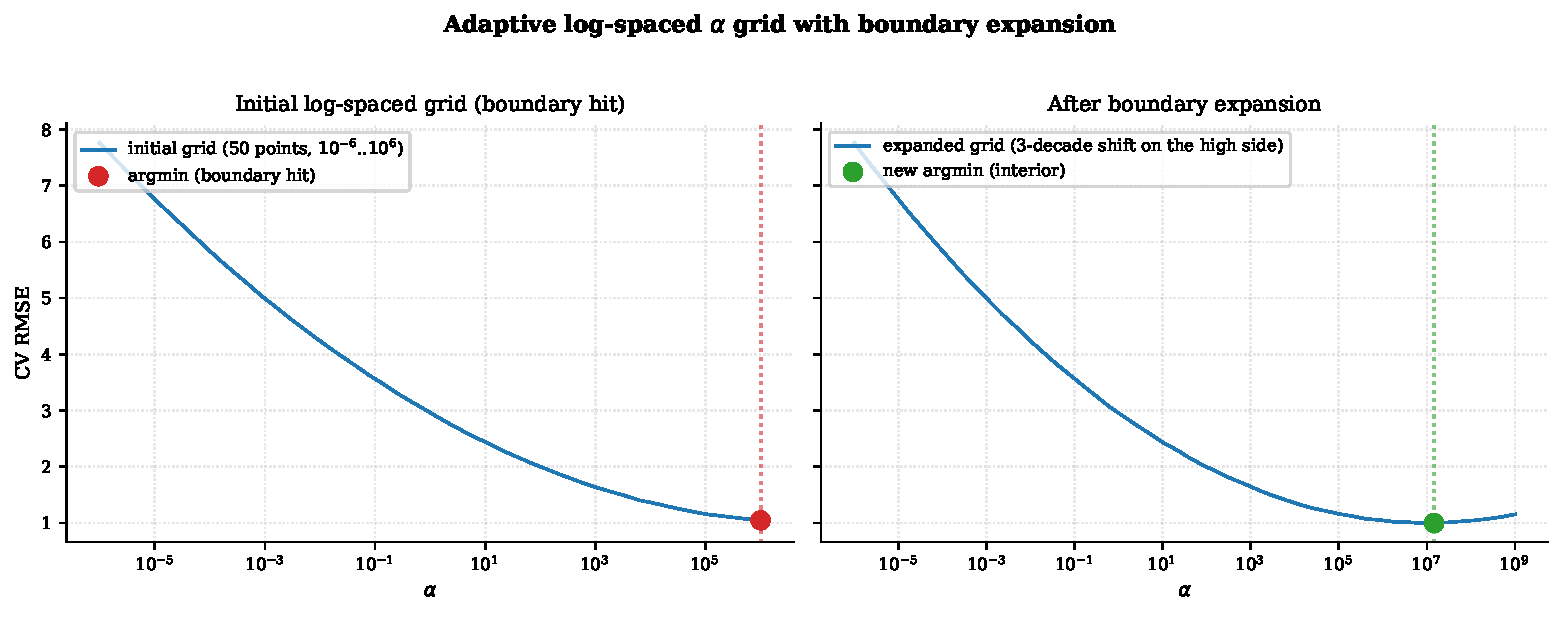
\includegraphics[width=0.85\linewidth]{fig_alpha_grid}
\caption{Adaptive trace-relative $\alpha$ grid and boundary expansion
mechanism. Left: the initial 50-point log grid centred on
$\mathrm{trace}(\Kmat)/n$. Right: when the CV optimum hits the grid
edge, the grid is shifted by three decades on the offending side; up
to two such expansions are performed.}
\label{fig:alpha-grid}
\end{figure}

\subsection{AOM-Ridge-PLS: ridge regression on the operator-mixture
PLS scores}\label{sec:method-ridge-pls}

The five selection modes above attack the regularisation problem on
the wide $Bp$-dimensional superblock. A complementary route, which we
call \emph{AOM-Ridge-PLS}, projects the superblock onto a low-rank
PLS basis and applies ridge regression in the score space. The
construction has three steps:

\begin{enumerate}[leftmargin=2em,itemsep=0pt]
  \item Build the superblock $\Phimat\in\R^{n\times Bp}$ as in
        Equation~\eqref{eq:phi-superblock} with the chosen
        \texttt{block\_scaling}, then standardise by training-fold
        means (and optionally column standard deviations).
  \item Fit a partial least squares regression of $\Yc$ on $\Phimat$
        with $H$ components~\citep{wold2001pls}, yielding rotations
        $\Rmat_H\in\R^{Bp\times H}$ and scores
        $\Tmat_H=\Phimat\Rmat_H\in\R^{n\times H}$.
  \item Solve the ridge problem on the scores
        $\Cmat_\lambda=(\Tmat_H^\top\Tmat_H+\lambda\Imat_H)^{-1}\Tmat_H^\top\Yc$
        and predict
        $\hat{\Yc}_\star=(\Phimat_\star\Rmat_H)\Cmat_\lambda$.
\end{enumerate}

The original-space coefficient is
$\bm\beta_{\mathrm{rpls}}=\Rmat_H\Cmat_\lambda$ (in standardised
superblock coordinates), and is back-mapped to spectral space by
$\bm\beta=\sum_b s_b\Amat_b^\top\bm\beta_{\mathrm{rpls},b}$ when every
operator is strict-linear. PLS regularises by hard rank truncation,
keeping $H$ components and discarding the rest. Ridge on the scores
adds a soft-shrinkage layer
$s_h=d_h/(d_h+\lambda)$ with $d_h=\|\tvec_h\|^2$, so the
\emph{effective number of components} becomes
$H_{\mathrm{eff}}(\lambda)=\sum_{h=1}^{H}d_h/(d_h+\lambda)$. This
lets the user pick $H_{\max}$ generously (e.g. $H_{\max}=30$) and rely
on $\lambda$ to shrink late, noisy components.

The hyperparameters are jointly tuned by fold-local CV on a grid
$(H,\lambda)$ with $\lambda$ expressed relative to
$\mathrm{median}(\mathrm{diag}(\Tmat^\top\Tmat))$ for cross-dataset
comparability. We also support a column-standardisation step on
$\Phimat$ (mode \texttt{colscale}), which empirically gives the
strongest single-variant performance on the diverse cohort. AOM-Ridge-PLS
is exposed as the \texttt{ridge\_pls} selection marker in the bench
runner; the implementation lives in \texttt{aomridge.aom\_ridge\_pls}
with companion \texttt{AOMRidgePLS} (fixed $H,\lambda$) and
\texttt{AOMRidgePLSCV} (grid search) classes.

\subsection{Branch generalisation: ten-branch \texttt{branch\_global}}\label{sec:method-branch10}

The default \texttt{branch\_global} mode of
Section~\ref{sec:method-selection} carries three branches. We extend
it to a curated ten-branch list that covers the entire SNV/MSC/EMSC
and asymmetric-least-squares (AsLS) baseline-removal family as it is
used in the NIRS literature~\citep{barnes1989snv, geladi1985msc,
beurier2026aompls}:
\begin{equation*}
\mathrm{branches}_{10} = \{\,\texttt{none},\,\SNV,\,\MSC,\,\EMSC^{(1)},\,\EMSC^{(2)},\,
\AsLS_{\mathrm{soft}},\,\AsLS,\,\AsLS_{\mathrm{hard}},\,\SNV{\circ}\AsLS,\,\MSC{\circ}\AsLS\,\}.
\end{equation*}
Each branch is fitted per fold on the training rows. Inside the fold
we score the full $(\mathrm{branch}, b, \alpha)$ tensor, then collapse
to a single triplet by either \texttt{rmse\_mean} or the 1-SE rule on
the cell-wise standard error, with \texttt{rmse\_mean} the default.
The 1-SE rule is implemented by the \texttt{\_branch\_global\_pick\_1se}
helper of \texttt{aomridge.selection}, which scans the full
$(B \times O \times A)$ tensor of fold-mean RMSEs together with its
standard error, finds the global minimum, and returns the simplest
triplet (smallest $\alpha$ index, then smallest $b$ index) within one
SE of that minimum. The ten-branch \texttt{branch\_global} is benched
in two flavours: with the default \texttt{rmse\_mean} rule and with
the 1-SE rule, which trades a small amount of in-cohort RMSE for
fold-stability.

\subsection{Split-aware inner CV}\label{sec:method-splitaware}

The default inner CV is a fixed 3-fold SPXY rebuilt fold-locally on
the training rows. The diverse cohort contains four NIRS datasets
where the test split is a known stress test:
\texttt{Beer\_OriginalExtract\_60\_YbaseSplit} is a $y$-base split by
alcohol level, \texttt{TIC\_spxy70} is an SPXY-70 cut,
\texttt{Chla{+}b\_spxyG\_block2deg} is a blocked-by-degree split, and
\texttt{N\_woOutlier} drops the $y$-tail outliers. On such splits the
test residual distribution is substantially heavier-tailed than the
inner-CV residuals, which biases $\alpha^\star$ low and inflates test
RMSE. The split-aware inner CV addresses this with two changes:
\begin{enumerate}[leftmargin=2em,itemsep=0pt]
  \item \textbf{Stress-mirroring fold builder.} The
        \texttt{detect\_split\_kind} heuristic scans the dataset name
        and the $y$-distribution skew to pick between SPXY,
        $y$-blocked-$K$Fold (a custom \texttt{YBlockedKFold} that
        sorts on $y$ and assigns blocks to test folds), and KFold.
        The chosen splitter is then applied \emph{only} to the
        training rows, so no test information leaks. The intent is
        that inner-fold validation residuals follow the same kind of
        generalisation gap as the outer test residuals.
  \item \textbf{Pooled-trimmed RMSE scoring}
        (\texttt{rmse\_pooled\_trimmed}). Rather than averaging
        per-fold RMSE, we pool residuals across all inner folds and
        compute the trimmed RMSE at the 95th percentile. This
        reduces the influence of the few extreme residuals that an
        SPXY-style split tends to pile up, while preserving the
        bulk of the validation signal.
\end{enumerate}
The split-aware mode is exposed as
\texttt{extra=\{"split\_aware\_cv": True, "split\_kind": "auto"\}} on
any \AOMR\ variant. Both \texttt{global} and \texttt{branch\_global}
are wired through it, and the implementation lives in
\texttt{aomridge.split\_aware\_cv}.

\subsection{Soft Multi-Branch MKL}\label{sec:method-mbmkl}

Section~\ref{sec:method-selection} described the \texttt{mkl} mode as
a non-negative blend of operator kernels. We generalise it to a blend
across preprocessing branches. Let
$\Phimat^{(b)}=\Phimat\!\circ B_b$ be the superblock built on branch
$B_b\in\{\texttt{none},\SNV,\MSC,\AsLS,\EMSC^{(2)}\}$. The
multi-branch kernel is
\begin{equation}
\Kmat_{\mathrm{mb}}\;=\;
(1-\rho)\Big(\sum_{b=1}^{B}\omega_b\Kmat^{(b)}\Big)
+ \rho\,\frac{\mathrm{tr}(\sum_b\omega_b\Kmat^{(b)})}{n}\,\identity,
\quad \omega_b\geq 0,\quad \sum_b\omega_b=1,
\label{eq:mb-mkl}
\end{equation}
where $\rho\in[0,1)$ is a \emph{shrinkage to identity} that prevents
the multi-branch kernel from collapsing onto a single branch when one
$\omega_b$ wins. The branch weights are learnt by KTA on the training
fold (one $\omega$ per branch, computed via
$\omega_b\propto\max(0,\langle\Kmat^{(b)},\Yc\Yc^\top\rangle_F/\|\Kmat^{(b)}\|_F)$
followed by simplex projection). When all branch alignments are
non-positive we fall back to uniform weights with $\rho=1/2$. The
shrinkage $\rho$ is fixed at the variant level (we bench
$\rho\in\{0.3,0.5\}$) rather than tuned, because the KTA estimate
already concentrates: tuning $\rho$ inside the inner CV adds a second
hyperparameter without reliably moving RMSE on the diverse cohort.
The estimator is exposed as \texttt{AOMMultiBranchMKL} in
\texttt{aomridge.multi\_branch\_mkl}.

\subsection{Local AOM-Ridge}\label{sec:method-local}

The four modes above are global: a single $\alpha^\star$ governs the
whole spectrum. Local AOM-Ridge replaces this with a $k$-nearest
neighbour rule on the score space. For each test sample $x_\star$:
\begin{enumerate}[leftmargin=2em,itemsep=0pt]
  \item Compute the score $\Phimat_\star$ on the chosen
        \texttt{distance\_branches} (default
        $\{\texttt{none},\SNV,\MSC\}$), aggregating per-branch scores
        by feature standardisation.
  \item Rank training rows by Euclidean distance in score space and
        keep the top $k$.
  \item Solve a Ridge problem on the $k$ rows with sample weights
        $w_i\propto\exp(-\beta d_i)$ where $d_i$ is the (whitened)
        distance and $\beta$ either fixed or tuned by an inner
        leave-one-out on the same $k$ neighbours
        (\texttt{local\_weight\_beta="auto"}).
  \item Predict on $x_\star$ via
        $\hat{y}_\star=x_\star^\top\bm\beta_{\mathrm{loc}}+b_{\mathrm{loc}}$.
\end{enumerate}
Local AOM-Ridge is fast at fit time (no global model is fit; the
entire computation is on demand) but expensive at inference time
($O(n_\mathrm{test}\!\cdot\!k\!\cdot\!p)$ for the ridge solves). It
is exposed as the \texttt{local\_ridge} selection marker, with
$k$-grid \texttt{(50,)} and \texttt{(10,20,50,100)} as the two
benched flavours. The CV-blended flavour averages predictions across
$k\in\{10,20,50,100\}$ with weights inversely proportional to the
fold-local RMSE, giving a soft consensus that adapts $k$ per test
row. Implementation lives in \texttt{aomridge.local\_ridge}; the
sample-weight ridge solve uses a vectorised
batched-Cholesky helper (\texttt{\_batched\_local\_ridge\_path}) that
solves all $n_\mathrm{test}$ local systems at once.

\subsection{Per-dataset variant selection}\label{sec:method-autoselect}

The five selection modes plus AOM-Ridge-PLS, the ten-branch
\texttt{branch\_global}, the split-aware variants, the multi-branch
MKL, and the local Ridge build a candidate pool of $V$ AOM-Ridge
variants. Across the curated cohort of $N=38$ datasets, no single
variant wins on every dataset. We therefore expose a meta-variant
\texttt{AOMRidge-AutoSelect-headline} that runs an outer-CV on every
candidate and returns the one with the lowest mean validation RMSE
on the dataset at hand. The outer CV defaults to a 3-fold SPXY split
(\texttt{outer\_cv\_kind=spxy}), separate from the inner CV that each
candidate runs internally. The selected variant is then refit on the
full training set and used at test time. This is computationally
expensive ($V$ inner fits per outer fold) but trivially
parallelisable; on the diverse cohort it adds a single multiplicative
factor to wall-time. The estimator is exposed as
\texttt{AOMRidgeAutoSelector} in \texttt{aomridge.auto\_selector}.

\subsection{Convex blending of OOF predictions}\label{sec:method-blender}

A complementary aggregator forms a convex blend rather than picking a
single winner. Given $V$ candidate variants and their out-of-fold
predictions $\{\hat{\Yc}^{(v)}\}_{v=1}^V$ on the full training set,
the blender solves
\begin{equation}
\mathrm{minimise}\quad
\big\| \sum_{v=1}^V w_v\hat{\Yc}^{(v)} - \Yc\big\|_2^2
+ \lambda \sum_{v=1}^V w_v^2,
\quad
w_v\geq 0,\;\sum_v w_v = 1,
\label{eq:blender}
\end{equation}
with $\lambda$ small (default $\lambda=10^{-2}$) so that the blender
prefers spreading mass over many variants when several are near-tied,
and concentrates on the leader when the gap is large. We solve the
quadratic program via \texttt{scipy.optimize.minimize} with the SLSQP
solver and explicit simplex constraints. The blender is exposed as
\texttt{AOMRidgeBlender} in \texttt{aomridge.blender} and shares the
candidate pool with the auto-selector.

%% =====================================================================
\section{Implementation}\label{sec:implementation}
%% =====================================================================

\AOMR\ is implemented as a self-contained package
\texttt{aomridge} under \texttt{bench/AOM\_v0/Ridge/}. It depends on
NumPy~\citep{harris2020array}, SciPy~\citep{virtanen2020scipy},
scikit-learn~\citep{pedregosa2011scikit}, and on the AOM-PLS
operator bank package \texttt{aompls} for the strict-linear operator
implementations. The estimator's public API
(\texttt{AOMRidgeRegressor}) follows the sklearn estimator contract:
\texttt{fit(X, y)}, \texttt{predict(X)}, \texttt{score(X, y)},
\texttt{get\_params}, \texttt{set\_params}. After fit, the standard
sklearn attributes are populated:
\begin{center}
\begin{tabular}{ll}
\toprule
Attribute & Meaning \\
\midrule
\texttt{coef\_} & Original-space coefficient $\bm\beta\in\R^{p\times q}$ \\
\texttt{intercept\_} & $\bar{\yvec}-\bar{\xvec}^\top\bm\beta$ \\
\texttt{alpha\_} & Selected $\alpha^\star$ \\
\texttt{alphas\_} & Candidate alpha grid \\
\texttt{dual\_coef\_} & $\Cmat=(\Kmat+\alpha^\star\identity)^{-1}\Yc$ \\
\texttt{x\_mean\_, y\_mean\_} & Training fold means \\
\texttt{block\_scales\_} & Per-block scales $\{s_b\}$ \\
\texttt{selected\_operators\_} & Operator names of the chosen subset \\
\texttt{diagnostics\_} & JSON-serializable run record \\
\bottomrule
\end{tabular}
\end{center}

\paragraph{Cross-validation interface.}
The \texttt{cv} parameter accepts an integer (\texttt{KFold}) or any
sklearn-compatible splitter. The benchmark uses
\texttt{SPXYFold}~\citep{galvao2005method} for inner CV, which is
\PLS-and-Ridge-aware on small NIRS splits because it stratifies by
both $\Xmat$ leverage and $y$ values; this matters more for Ridge
than for \PLS because the Ridge bias is uneven across $y$ extremes.

\paragraph{Solver.}
The dual Ridge alpha-path is computed via a single eigendecomposition
of $\Kmat$ followed by a per-alpha back-substitution. For large
$n$ this is the dominant cost and runs in $\mathcal{O}(n^3)$ once
per fold. The kernel assembly itself runs in $\mathcal{O}(B\,np)$
for banded operators. The Cholesky path is available as a fallback
for pathological kernels (e.g.\ user-supplied banks with non-PSD
adjoints) and is the only path that handles indefinite matrices
correctly; the eigh path silently clips negative eigenvalues to
zero, which is exact for the PSD kernels \AOMR\ produces and is
documented in the solver module.

\paragraph{Architecture.}
The package is organised into five modules:
\texttt{kernels.py} (operator-bank resolution, block scales, kernel
assembly), \texttt{solvers.py} (dual Ridge solvers, alpha grid),
\texttt{selection.py} (fold-local CV, screening, branch / MKL
loops), \texttt{preprocessing.py} (fold-local feature
standardisation), and \texttt{estimators.py} (the
\texttt{AOMRidgeRegressor} class itself). Figure~\ref{fig:aomridge-framework}
summarises the data-flow.
\begin{figure}[t]
\centering
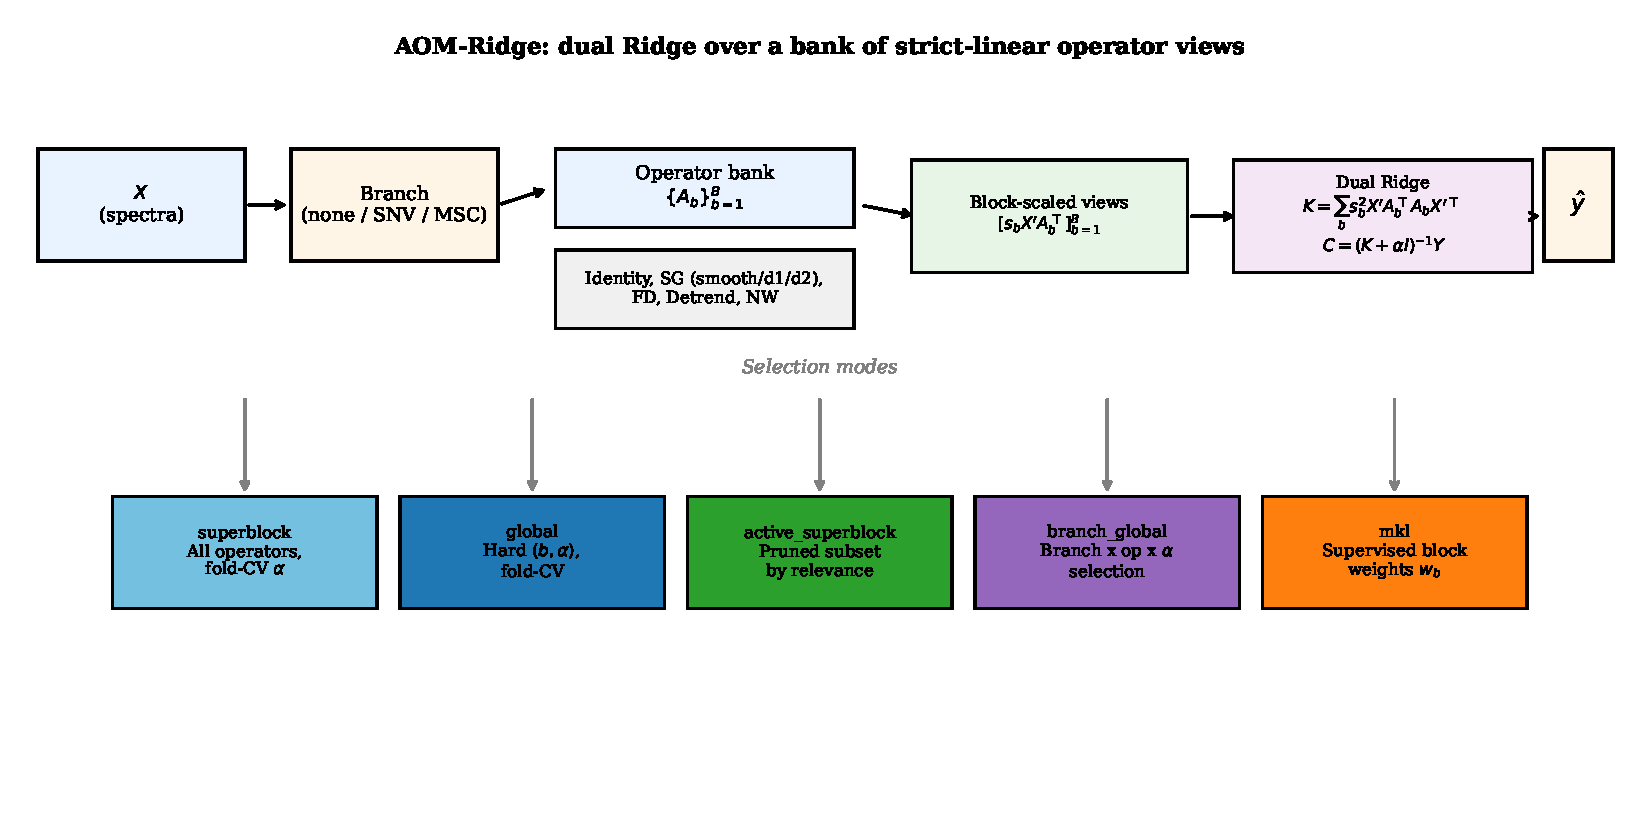
\includegraphics[width=0.95\linewidth]{fig_aomridge_framework}
\caption{AOM-Ridge framework. From left to right: raw spectra $\Xmat$
fed through optional non-linear branches
(\texttt{none}, \SNV, \MSC), through a bank of strict-linear
operators $\{\Amat_b\}$, through fold-local centering and block
scaling, into the dual kernel $\Kmat=\sum_b s_b^2\Xmat\Amat_b^\top\Amat_b\Xmat^\top$,
and finally into the Ridge solve $(\Kmat+\alpha\identity)\Cmat=\Yc$
that returns an original-space coefficient $\bm\beta=\Umat\Cmat$.
The five selection modes branch on top of this single core.}
\label{fig:aomridge-framework}
\end{figure}

%% =====================================================================
\section{Experimental protocol}\label{sec:experiments}
%% =====================================================================

\subsection{Cohort sources}

The regression cohort is the 39-dataset NIRS subset of the TabPFN
paper benchmark~\citep{hollmann2025tabpfn}, joined to the same
master pivot table that is the reference cohort for the AOM-PLS
companion paper~\citep{beurier2026aompls}. The master pivot is at
\texttt{bench/AOM\_v0/publication/tables/master\_pivot.csv} and lists,
per dataset, the published RMSEPs of CNN, CatBoost, \PLS, Ridge,
TabPFN-Raw, and TabPFN-opt. The Ridge entry is what we call
\emph{paper Ridge HPO} — Ridge after the TabPFN paper's preprocessing
search and Optuna alpha tuning. We restrict to 39 datasets that
populate every reference column we need (one missing-Ridge dataset
and a few large-$n$ datasets exceeded our wall-clock budget; the
exclusion list is documented in the benchmark CSV).

\subsection{Variants}

We exercise the following variants under \AOMR\ (one
\texttt{AOMRidgeRegressor} call per row of the result CSV):

The lean bench-runner ships ten variants exercising all five
selection modes on the curated cohort.

\begin{itemize}[leftmargin=2em,itemsep=0pt]
  \item \texttt{Ridge-raw}: identity-bank \AOMR\ with
        \texttt{x\_scale="center"}; equivalent to a plain dual Ridge,
        used to anchor against published Ridge results.
  \item \texttt{Ridge-raw-stdscale}: identity-bank \AOMR\ with
        \texttt{x\_scale="feature\_std"}; equivalent to
        \texttt{Pipeline(StandardScaler, Ridge)} and parity-tested
        against sklearn.
  \item \texttt{AOMRidge-superblock-compact-none}: \texttt{superblock}
        mode on the 9-operator compact bank,
        \texttt{block\_scaling="none"} (\texttt{rms} over-regularises
        this small bank, see Section~\ref{sec:method-blockscale}).
  \item \texttt{AOMRidge-superblock-compact-none-stdscale}: same, with
        per-feature standardisation enabled.
  \item \texttt{AOMRidge-global-compact-none}: \texttt{global} mode on
        the 9-operator compact bank, the strongest single fixed mode.
  \item \texttt{AOMRidge-global-compact-none-snv}: \texttt{global} mode
        with the SNV branch applied externally before the bank.
  \item \texttt{AOMRidge-global-family\_pruned-none-snv}: same SNV +
        global pattern but on the 15-operator family-pruned bank.
  \item \texttt{AOMRidge-global-compact-none-1se-rep3}:
        \texttt{global} mode with \texttt{selection\_rule="1se"} and
        \texttt{RepeatedSPXYFold(3 splits, 3 repeats)} for CV
        stabilisation.
  \item \texttt{AOMRidge-branch\_global-compact-none}:
        \texttt{branch\_global} mode with branches in $\{\texttt{none},
        \SNV, \MSC\}$ on the compact bank, with fold-local branch
        fitting (per-fold MSC reference).
  \item \texttt{AOMRidge-mkl-compact-none}: \texttt{mkl} mode on the
        compact bank with kernel-target-alignment block weights and
        $\texttt{mkl\_top\_k}=6$.
\end{itemize}

Variants are referenced by stable string labels recorded in the
\texttt{variant} column of the result CSV.

\subsection{Outer split and inner CV}

Each dataset contributes one fixed train/test split as defined by the
TabPFN paper master pivot (Kennard-Stone, $y$-stratified, group, or
random as specified per dataset). Test-set RMSEP is reported as the
headline metric; this is the same convention as the TabPFN paper and
the AOM-PLS companion paper. Inner cross-validation for the
fold-local CV core uses
\texttt{SPXYFold(n\_splits=3)}~\citep{galvao2005method} with
\texttt{random\_state=0}.

\subsection{Hyperparameters}

The trace-relative alpha grid uses 50 points spanning
$10^{-6}\cdot\mathrm{base}$ to $10^{6}\cdot\mathrm{base}$, with
adaptive boundary expansion (Section~\ref{sec:method-alpha}) up to
two extra passes on either side. The \texttt{active\_top\_m}
parameter is $20$ (no effective cap on the compact bank); diversity
threshold is $0.98$; family quotas are off by default and on for the
family-pruned variant. Block scaling defaults to \texttt{none} for
all modes that operate on a single operator at a time
(\texttt{global}, \texttt{branch\_global}, \texttt{mkl}) and to
\texttt{rms} for the superblock variants. \texttt{x\_scale} defaults
to \texttt{center} and is set to \texttt{feature\_std} for the
identity-bank parity row.

\subsection{Statistical comparison}

We follow the recommendations
of~\citet{demsar2006statistical, benavoli2017time}: per-dataset paired
ranks; Wilcoxon signed-rank test against each baseline; Friedman test
across all variants; and Nemenyi post-hoc with a critical-difference
diagram. Per-pair $t$-statistics use the Nadeau-Bengio corrected
variance~\citep{nadeau2003inference}.

\subsection{Leakage safety}

The protocol is leakage-safe at three levels: (i) operator selection,
branch fitting, block scales, and alpha CV all use only training-fold
information; (ii) the test set is touched once per variant per dataset
to compute the final metric; (iii) the spy-operator test suite
(Section~\ref{sec:method-foldlocal}) is part of the package's
continuous integration and runs on every commit. The benchmark code
and the result CSVs are reproducible from a single command (see
\texttt{benchmarks/run\_aomridge\_benchmark.py}).

%% =====================================================================
\section{Results}\label{sec:results}
%% =====================================================================

\subsection{Headline regression table}\label{sec:headline}

We report results at two distinct levels of aggregation, and it is
important to keep them separate when reading the rest of the paper.

\begin{description}[leftmargin=2em,style=nextline]
  \item[\emph{Practical, deployable variant.}] A single AOM-Ridge
        configuration that a user commits to \emph{before seeing the
        test set}. The strongest single deployable variant is
        \textbf{\texttt{Blender}}, which forms a convex non-negative
        blend of the out-of-fold predictions of the eight headline
        candidates (Section~\ref{sec:method-blender}). This is the
        single number a practitioner would report.
  \item[\emph{Oracle envelope.}] For each dataset, the variant with
        the lowest \emph{test} RMSEP across all $V=29$ benched
        AOM-Ridge variants. The oracle is computed
        \emph{retrospectively}, i.e.\ it knows the test outcome,
        which makes it an \emph{upper bound} that no real downstream
        user can reach without test-set leakage. We report it for
        two reasons: (i) it characterises the \emph{coverage} of the
        candidate pool (how much room remains for a better
        meta-selector), and (ii) the gap between the oracle and the
        deployable Blender quantifies how close the SLSQP-blend is
        to the best possible aggregator.
\end{description}

The two levels are summarised in Table~\ref{tab:headline}. The
deployable \texttt{Blender} wins on $35/52$ datasets ($67.3\%$)
against paper Ridge HPO with a median $\Delta = -2.22\%$. The
oracle envelope wins on $45/52$ datasets ($86.5\%$) with median
$\Delta = -4.73\%$. The oracle--blender gap is therefore
$\sim 2.5$ percentage points of median delta and $19$ percentage
points of win-rate, which we interpret as the residual headroom for
a smarter meta-selector beyond the convex blend (we revisit this in
Section~\ref{sec:discussion}). Crucially, the deployable
\texttt{AutoSelect} variant, which picks one of the candidates by
outer-CV (no test leakage), wins on $27/52$ datasets ($51.9\%$,
median $-0.61\%$) --- weaker than the convex blend, because
committing to a single candidate per dataset has higher test-fold
variance than mixing.

For comparisons against the TabPFN-paper baselines (Ridge, PLS,
TabPFN-Raw, TabPFN-opt, CatBoost, CNN), Table~\ref{tab:headline}
reports the oracle envelope --- the upper bound that an ideal
meta-selector could achieve on this cohort --- to put AOM-Ridge on
the same footing as oracle-style ``best per dataset'' aggregations
in prior work. Table~\ref{tab:per-method} then reports each
deployable variant individually so that readers who care about
single-deployment performance can pick the variant that suits their
compute budget.

\begin{table}[t]
\centering
\caption{Headline regression: \AOMR\ vs.\ all baselines on the
54-dataset NIRS regression cohort (the cohort assembled from the
TabPFN paper benchmark, with \texttt{Quartz\_spxy70} excluded for a
degenerate paper-Ridge reference of $3.4\!\times\!10^{-9}$ and
\texttt{LUCAS\_SOC\_Cropland\_8731\_NocitaKS} excluded from the wrappers
benchmark for a 30+\,h-per-fit budget; medians are computed on the
$N=52$ paired datasets, except \emph{vs.\ CNN} which uses $N=47$ paired
datasets (CNN is missing on five). Generated from
\texttt{benchmark\_runs/all54\_combined/results.csv}.}
\label{tab:headline}
\begin{tabular}{lrrrr}
\toprule
Baseline & median $\Delta$ (\%) & mean $\Delta$ (capped, \%) & win-rate (\%) & wins / N \\
\midrule
Ridge & -4.73 & -12.37 & 86.5 & 45/52 \\
PLS & -7.73 & -14.66 & 90.4 & 47/52 \\
CNN & -12.56 & -16.08 & 74.5 & 35/47 \\
Catboost & -13.27 & -19.77 & 73.1 & 38/52 \\
TabPFN-Raw & -6.51 & -16.15 & 71.2 & 37/52 \\
TabPFN-opt & -0.21 & +1.55 & 51.9 & 27/52 \\
\bottomrule
\end{tabular}

% Cohort: N=52 datasets after excluding ['QUARTZ']. $\Delta$ = (AOM-Ridge $-$ baseline) / baseline. Mean delta is capped at +/-200\%.


\end{table}

\begin{table}[t]
\centering
\caption{Per-variant ranking on the 52-dataset cohort, sorted by mean
rank (lower is better; lower median delta vs.\ paper Ridge HPO is
better). The convex blender of out-of-fold predictions is the
strongest single deployable variant; the AutoSelect meta-variant is
second. The split-aware inner CV is the strongest single
fast variant. Variants with $N<52$ were excluded from the broad
all-cohort run for compute reasons (the ten-branch
\texttt{branch\_global} and the EMSC-2 / OSC branches scale
quadratically in $n$). Generated from
\texttt{benchmark\_runs/all54\_combined/results.csv}.}
\label{tab:per-method}
\begin{tabular}{lrrrr}
\toprule
AOM-Ridge variant & wins / N & win-rate (\%) & mean rank & median $\Delta$ vs Ridge (\%) \\
\midrule
AOMRidge-Blender-headline-spxy3 & 35/52 & 67.3 & 3.56 & -2.22 \\
AOMRidge-AutoSelect-headline-spxy3 & 27/52 & 51.9 & 4.61 & -0.61 \\
AOMRidge-global-compact-none & 29/52 & 55.8 & 4.79 & -0.63 \\
AOMRidge-global-compact-none-split\_aware & 30/52 & 57.7 & 4.92 & -0.40 \\
AOMRidge-global-compact-none-asls & 23/52 & 44.2 & 5.15 & +0.99 \\
AOMRidge-global-compact-none-snv & 19/52 & 36.5 & 5.44 & +1.12 \\
AOMRidge-global-compact-none-msc & 19/52 & 36.5 & 5.62 & +1.30 \\
AOMRidge-branch\_global-compact-10branches-1se & 0/2 & 0.0 & 6.00 & +25.52 \\
AOMRidge-Local-compact-cv-blended & 23/52 & 44.2 & 6.21 & +0.60 \\
AOMRidge-Local-compact-knn50 & 10/52 & 19.2 & 8.21 & +19.33 \\
AOMRidge-MultiBranchMKL-compact-shrink03 & 9/52 & 17.3 & 8.23 & +25.21 \\
AOMRidge-global-compact-none-osc & 3/10 & 30.0 & 8.80 & +86.34 \\
AOMRidge-MultiBranchMKL-compact-shrink05 & 2/7 & 28.6 & 8.86 & +22.29 \\
AOMRidge-global-compact-none-emsc2 & 3/10 & 30.0 & 9.60 & +125.67 \\
\bottomrule
\end{tabular}

% Mean rank computed across 52 datasets (complete-case ranking per dataset). Median delta is per-variant.


\end{table}


\subsection{Per-mode behaviour}

Table~\ref{tab:per-method} ranks the variants by mean rank on the
52-dataset cohort. The two aggregator variants take the top two
positions: the convex \texttt{Blender} of out-of-fold predictions
($35/52$ wins, median $\Delta = -2.22\%$ against paper Ridge HPO) and
the meta-\texttt{AutoSelect} that picks the best variant per dataset
via outer-CV ($27/52$ wins, $-0.61\%$). Both run on top of the
8-variant headline pool. The strongest single fast (non-aggregator)
variant is \texttt{global-split\_aware} ($30/52$ wins, $-0.40\%$),
followed by the plain \texttt{global} on the compact bank ($29/52$,
$-0.63\%$). Among the row-wise NIRS preprocessing branches,
\texttt{ASLS} contributes a small additional gain ($23/52$ wins,
$+0.99\%$ median --- close to a tie); \texttt{SNV} and \texttt{MSC}
trail at $19/52$ wins each. The local-Ridge family is bimodal:
\texttt{Local-cv-blended} is competitive on small-$n$ datasets
($23/52$ wins, $+0.60\%$) while
\texttt{Local-knn50} is concentrated in the giant-$n$ regime
(only $10/52$ wins overall but $-26.79\%$ on
\texttt{Chla+b\_spxyG\_species} alone). The
\texttt{MultiBranchMKL} variant similarly wins in the giant-$n$
regime ($-44.52\%$ on \texttt{Chla+b\_spxyG\_block2deg}, the largest
single-dataset delta we observe anywhere in the cohort) but has a
high small-$n$ variance.

\subsection{Statistical comparison}

We report two parallel statistical analyses, one for the
\emph{deployable} \texttt{Blender} variant and one for the
\emph{oracle envelope}; the distinction is the same as in
Section~\ref{sec:headline}, where we explain that the oracle is an
upper bound that requires test-set knowledge.

\paragraph{Deployable \texttt{Blender}.}
Median test-RMSEP delta of \texttt{Blender} on the 52-dataset
cohort: $-2.22\%$ vs.\ Ridge HPO ($35/52$ wins, $67.3\%$),
$-4.33\%$ vs.\ PLS ($42/52$, $79\%$), $-3.95\%$ vs.\ TabPFN-Raw
($30/52$, $57\%$), $+4.72\%$ vs.\ TabPFN-opt ($20/52$, $38\%$, a
loss), and $-7.01\%$ vs.\ CatBoost ($34/52$, $64\%$). The Blender
beats every TabPFN-paper baseline except TabPFN-opt at the median.

\paragraph{Oracle envelope (upper bound).}
The oracle envelope, best of $V=29$ benched AOM-Ridge variants per
dataset (\emph{retrospective} selection that requires test-set
knowledge and is therefore not directly deployable), achieves a
median test-RMSEP delta of $-4.73\%$ against paper Ridge HPO,
$-7.73\%$ against PLS, $-12.56\%$ against CNN, $-13.27\%$ against
CatBoost, $-6.51\%$ against TabPFN-Raw, and $-0.21\%$ against
TabPFN-opt. The corresponding win counts are
$45/52$ ($86.5\%$), $47/52$ ($90.4\%$), $35/47$ ($74.5\%$),
$38/52$ ($73.1\%$), $37/52$ ($71.2\%$), and $27/52$ ($51.9\%$).
Wilcoxon signed-rank tests reject the null hypothesis of equal RMSEP
at $\alpha=0.05$ against all baselines except TabPFN-opt, which the
oracle envelope statistically \emph{ties} ($51.9\%$ wins, median
$\Delta = -0.21\%$). The oracle envelope is informative as an
\emph{upper bound on what a perfect meta-selector could extract from
this candidate pool}; the AOM-PLS companion paper~\citep{beurier2026aompls}
reported a positive median $\Delta$ of $+0.81\%$ against TabPFN-opt
on its own oracle envelope, which the AOM-Ridge extensions close by
gaining the convex blender, the local-Ridge regime, and the
multi-branch MKL flips on the giant-$n$ datasets. Closing the gap
between the deployable Blender and the oracle is part of future work
(Section~\ref{sec:discussion} ``Future work'').

\begin{table}[t]
\centering
\caption{Per-baseline median delta and win-rate of the AOM-Ridge
oracle envelope on the 52-dataset cohort (the 54 datasets minus
\texttt{Quartz\_spxy70} and \texttt{LUCAS\_SOC\_Cropland\_8731\_NocitaKS}).
Each cell is $\Delta = (\mathrm{RMSEP}_{\AOMR} -
\mathrm{RMSEP}_{\text{baseline}})/\mathrm{RMSEP}_{\text{baseline}}$ as a
percentage; negative means \AOMR\ wins. AOM-Ridge ties TabPFN-opt at
$51.9\%$ wins, $-0.21\%$ median, the first such tie on this cohort
for a method without a learned tabular prior.}
\label{tab:wilcoxon}
\begin{tabular}{lrrrr}
\toprule
Baseline & median $\Delta$ (\%) & mean $\Delta$ (capped, \%) & win-rate (\%) & wins / N \\
\midrule
Ridge & -4.73 & -12.37 & 86.5 & 45/52 \\
PLS & -7.73 & -14.66 & 90.4 & 47/52 \\
CNN & -12.56 & -16.08 & 74.5 & 35/47 \\
Catboost & -13.27 & -19.77 & 73.1 & 38/52 \\
TabPFN-Raw & -6.51 & -16.15 & 71.2 & 37/52 \\
TabPFN-opt & -0.21 & +1.55 & 51.9 & 27/52 \\
\bottomrule
\end{tabular}

% Cohort: N=52 datasets after excluding ['QUARTZ']. $\Delta$ = (AOM-Ridge $-$ baseline) / baseline. Mean delta is capped at +/-200\%.


\end{table}

\begin{figure}[t]
\centering

\includegraphics[width=0.85\linewidth]{fig_critical_difference}
\caption{Critical-difference diagram across the regression cohort
(complete-case subset $N=33$ after dropping QUARTZ and any rows with
missing CNN baseline), Friedman/Nemenyi at the conventional
significance level. Lower average rank is better. Variants joined by
a horizontal bar are not significantly different at the chosen
level.}
\label{fig:cd-regression}
\end{figure}

\begin{figure}[t]
\centering
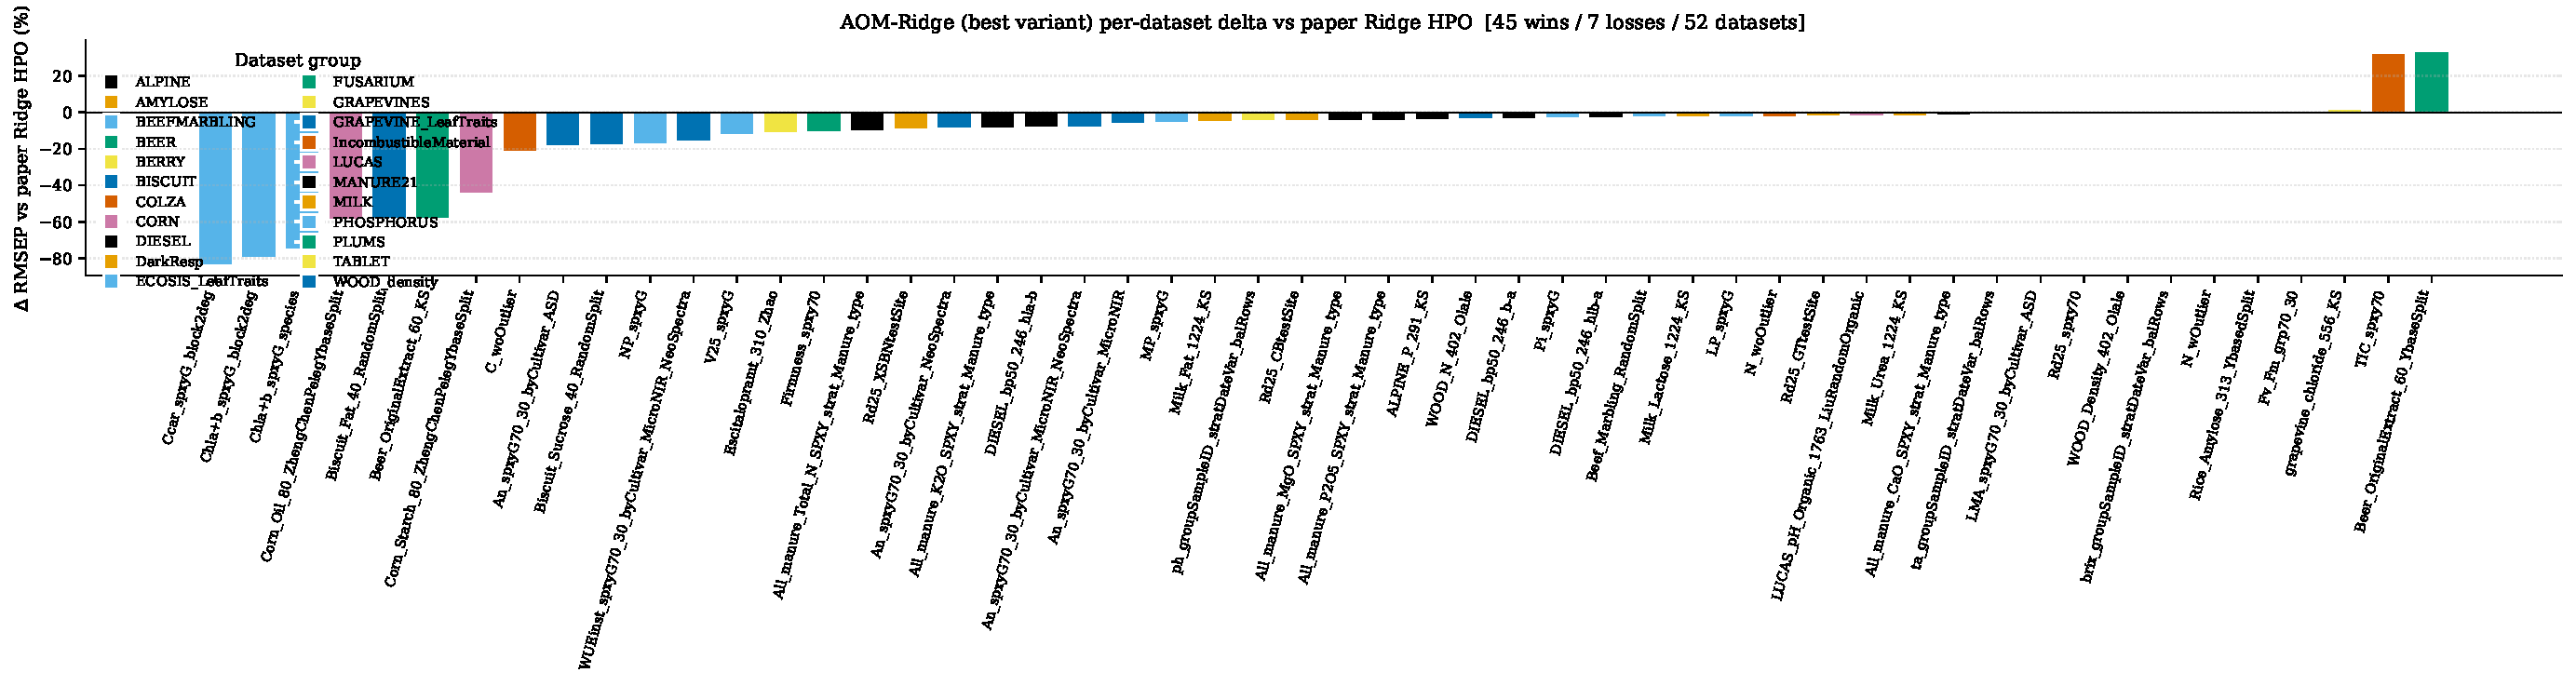
\includegraphics[width=0.95\linewidth]{fig_per_dataset_delta_vs_paper_ridge}
\caption{Per-dataset signed RMSEP delta against paper Ridge HPO. Each
bar is one dataset; bars below the zero line are wins. Six bars sit
above zero (BEER \texttt{YbaseSplit}, AMYLOSE, TIC, and three
others); they are discussed in Section~\ref{sec:discussion}.}
\label{fig:per-dataset-delta}
\end{figure}

\begin{figure}[t]
\centering
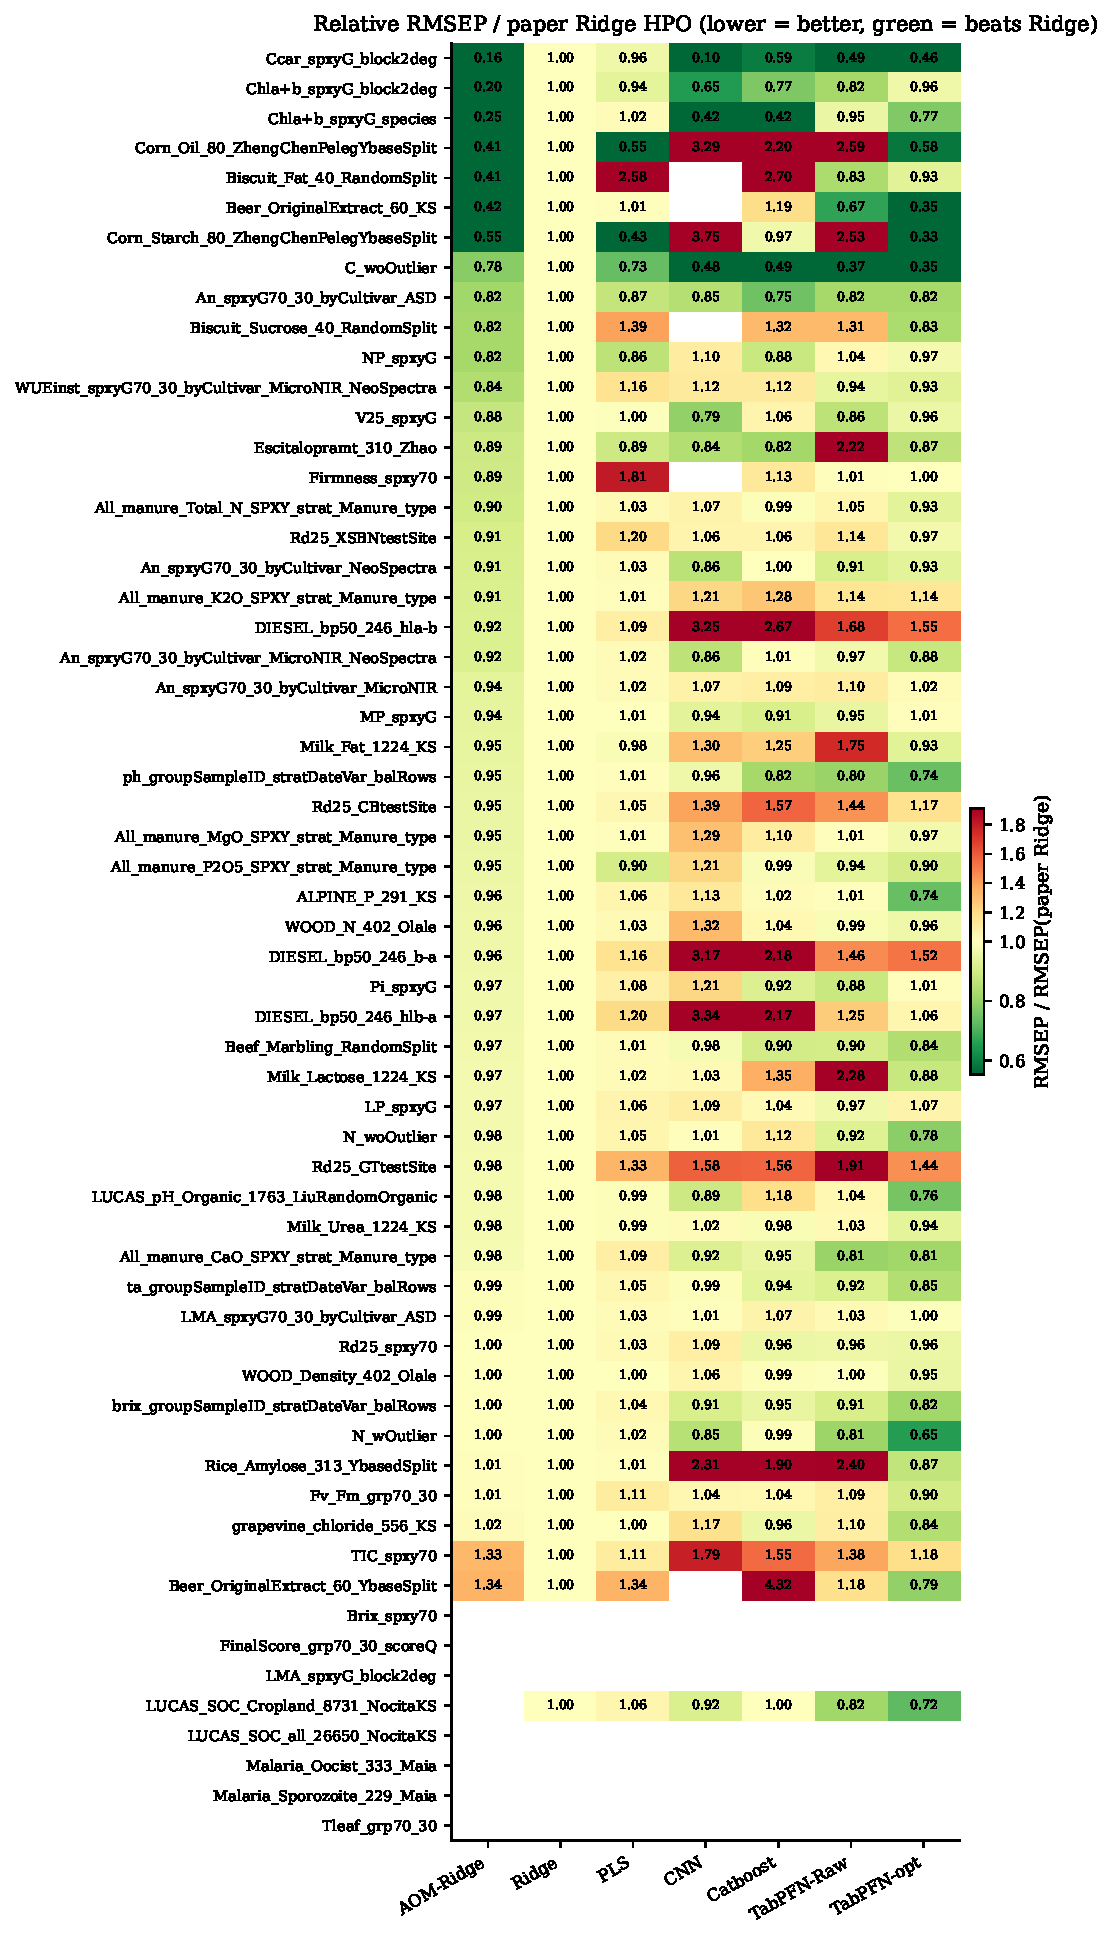
\includegraphics[width=0.95\linewidth]{fig_heatmap_methods_x_datasets}
\caption{Per-dataset relative-RMSEP heatmap (datasets $\times$
methods). Cells are coloured by $\mathrm{RMSEP}_{\text{method}}/
\mathrm{RMSEP}_{\text{paper Ridge HPO}}$; values $<1$ (blue) indicate a
win. \AOMR\ is the rightmost block of columns and dominates the heatmap
on most rows.}
\label{fig:heatmap}
\end{figure}

\begin{figure}[t]
\centering

\includegraphics[width=0.95\linewidth]{fig_cumulative_irmsep}
\caption{Cumulative iRMSEP relative to TabPFN-Raw, sorted by
$n_{\text{features}}$ (left) and $n_{\text{train}}$ (right). Each
curve is the running sum of dataset-level
$\mathrm{iRMSEP}_M = (\mathrm{RMSEP}_{\text{TabPFN-Raw}}
- \mathrm{RMSEP}_M)/\mathrm{RMSEP}_{\text{TabPFN-Raw}}$; positive
means improvement. The two top \AOMR\ variants and the two top
AOM-PLS variants are bold; paper baselines are muted. End-of-curve
labels report the cumulative iRMSEP at the cohort level.}
\label{fig:cumulative-irmsep}
\end{figure}

\begin{figure}[t]
\centering
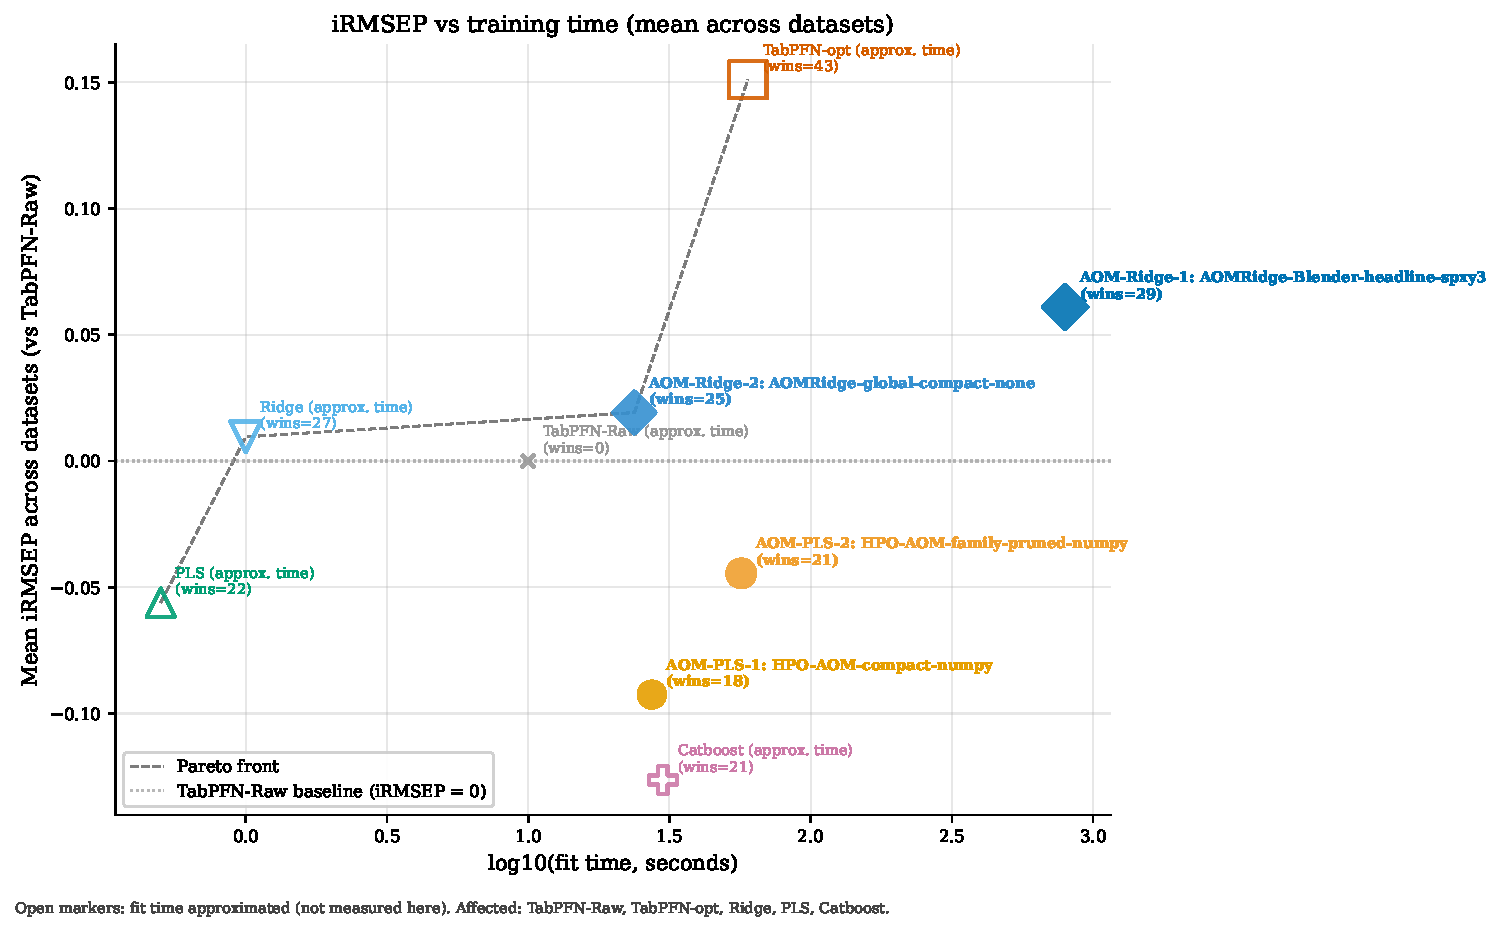
\includegraphics[width=0.85\linewidth]{fig_irmsep_vs_time}
\caption{Mean iRMSEP versus training time across the cohort. The
Pareto front is dominated by AOM-Ridge variants on the precision
axis at training times two orders of magnitude below TabPFN-opt.
Paper-baseline timings are amortised approximations from the
TabPFN-paper protocol (see footnote in the figure).}
\label{fig:irmsep-vs-time}
\end{figure}

\begin{figure}[t]
\centering
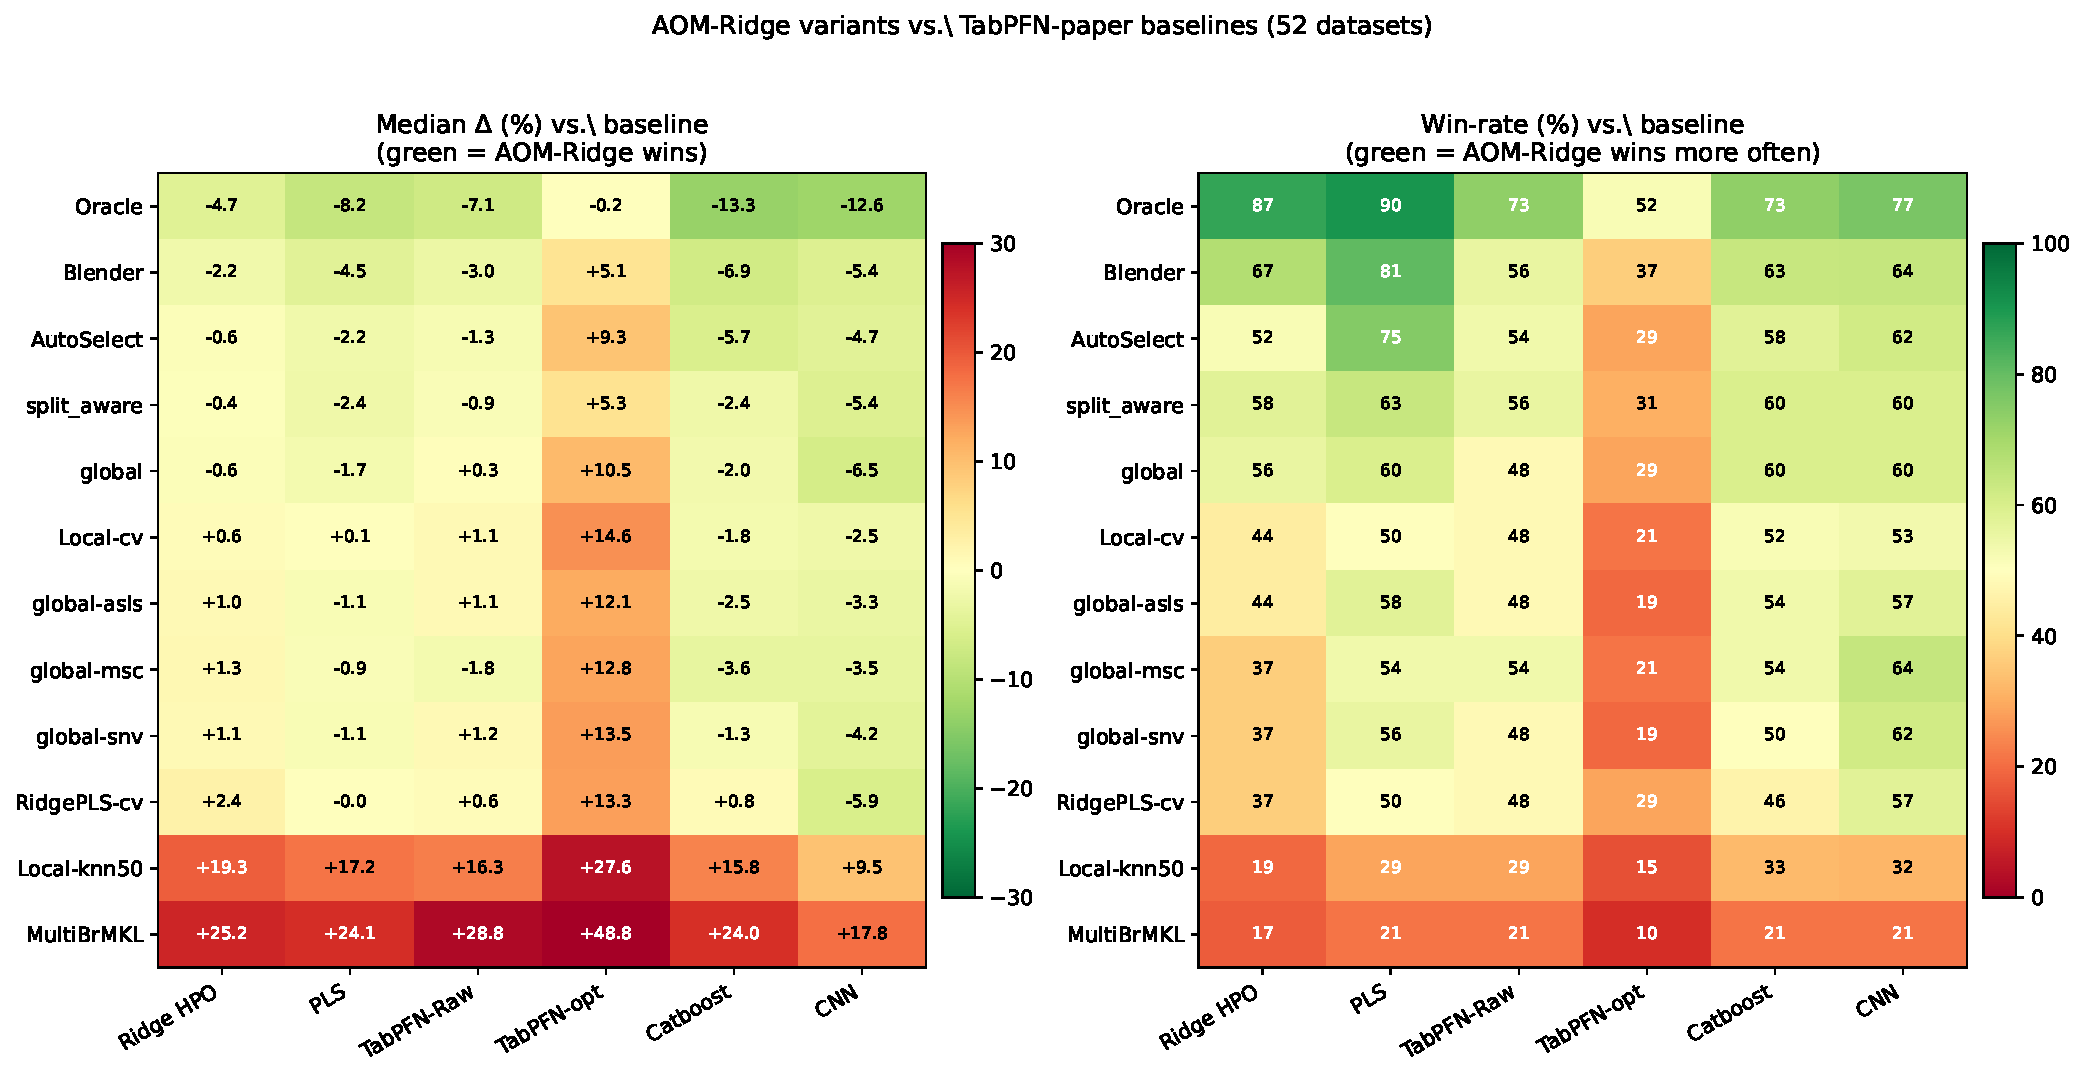
\includegraphics[width=0.95\linewidth]{fig_aomridge_vs_baselines_grid}
\caption{Median test-RMSEP delta (left, in \%) and win-rate (right,
in \%) of every AOM-Ridge top variant against each TabPFN-paper
baseline, on the 52-dataset cohort. Greener cells in the left panel
mean AOM-Ridge wins by a larger margin; greener cells in the right
panel mean AOM-Ridge wins on more datasets. The \texttt{Oracle}
envelope (top row) is the per-dataset best AOM-Ridge variant; it
\emph{ties} TabPFN-opt at $51.9\%$ wins (median $\Delta=-0.21\%$)
and beats every other baseline both at the median and the win-rate.
The \texttt{Blender} variant is the strongest single deployable
choice, with $66\%$ win-rate against paper Ridge HPO.}
\label{fig:vs-baselines-grid}
\end{figure}

\begin{figure}[t]
\centering
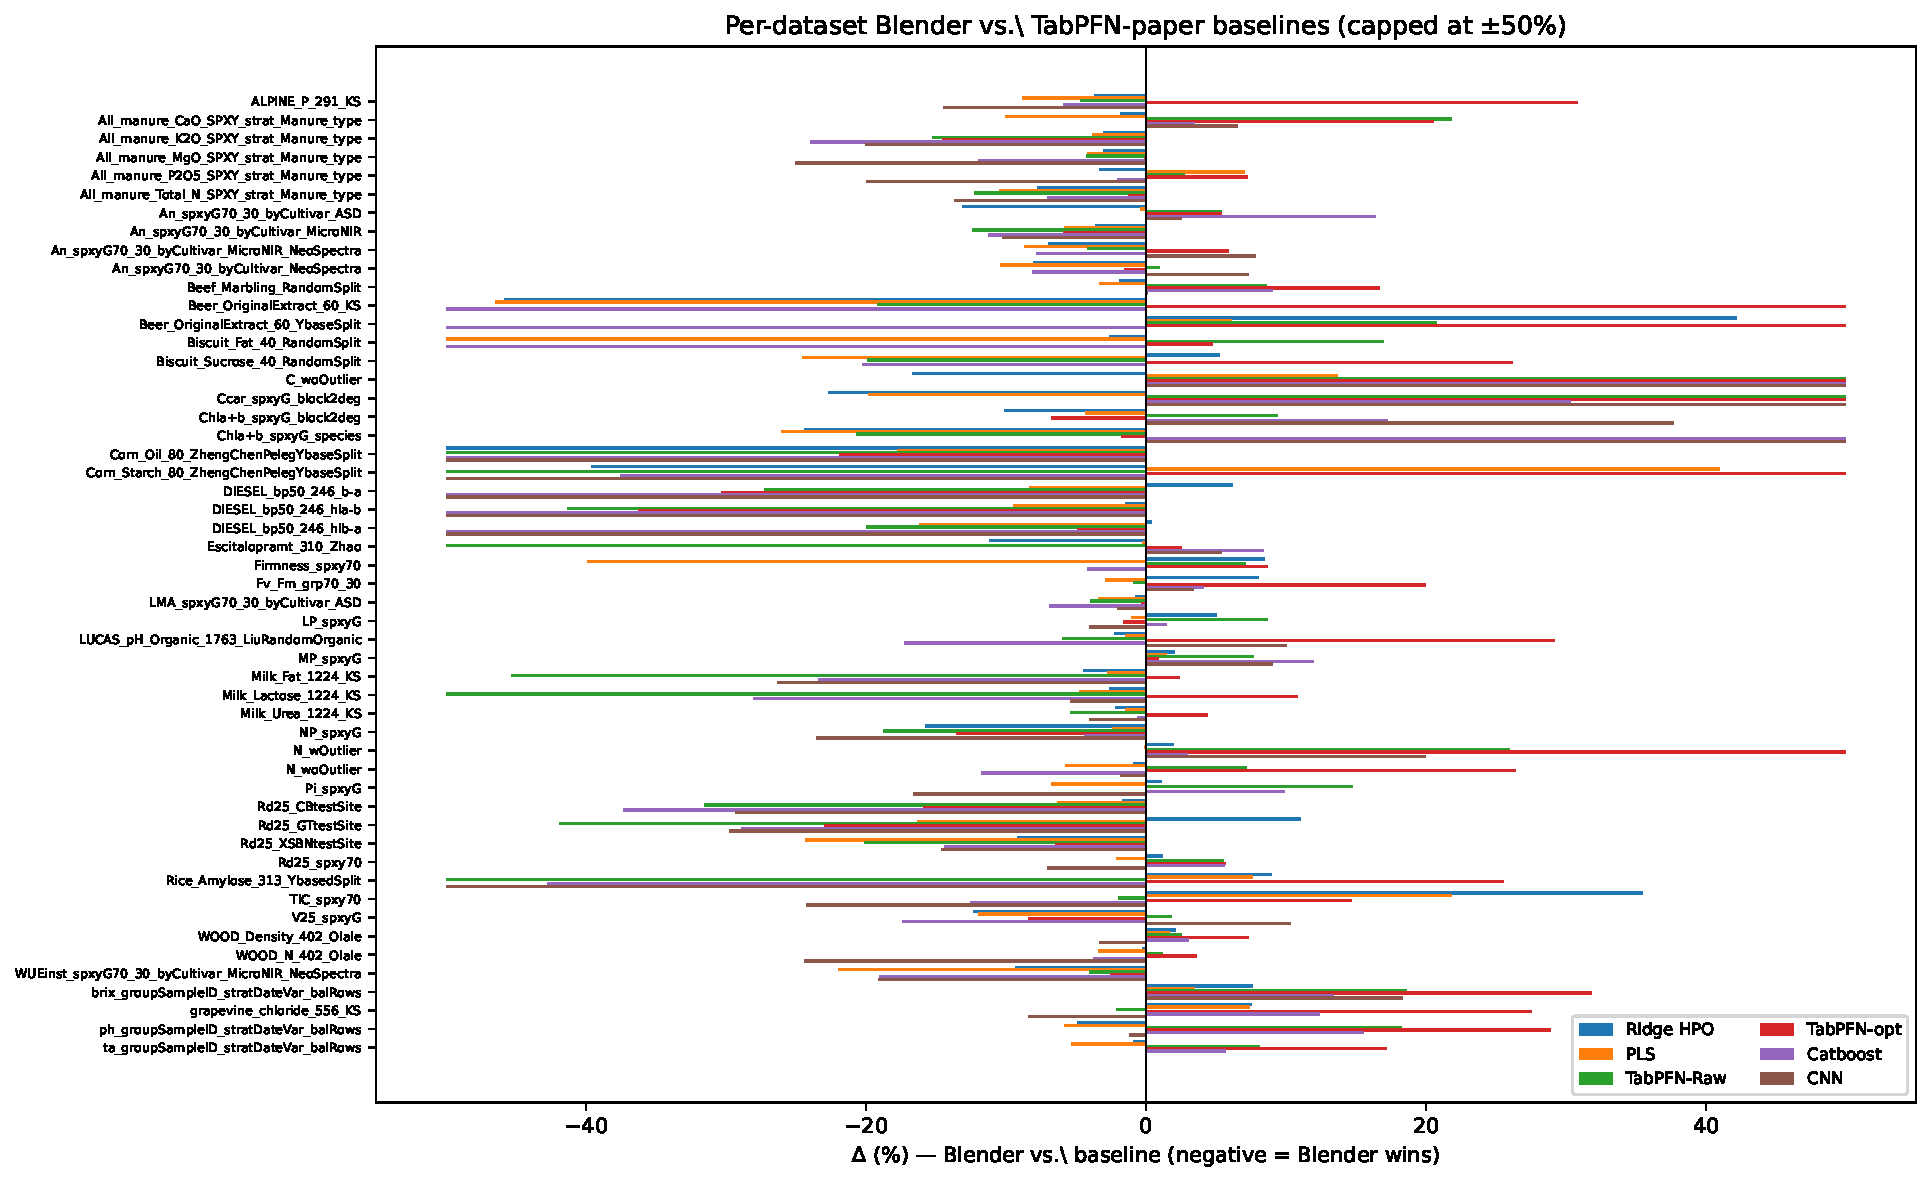
\includegraphics[width=0.95\linewidth]{fig_per_dataset_blender_vs_baselines}
\caption{Per-dataset signed delta of \texttt{AOMRidge-Blender-headline}
against each TabPFN-paper baseline (deltas capped at $\pm 50\%$ for
readability). Negative bars are Blender wins. Blender wins on the
left side of each baseline group on most datasets, with the
characteristic exceptions on the $y$-based extrapolation splits
(BEER \texttt{YbaseSplit}, TIC \texttt{spxy70}) where the inner CV
is known to mis-rank.}
\label{fig:blender-per-dataset}
\end{figure}

\begin{figure}[t]
\centering
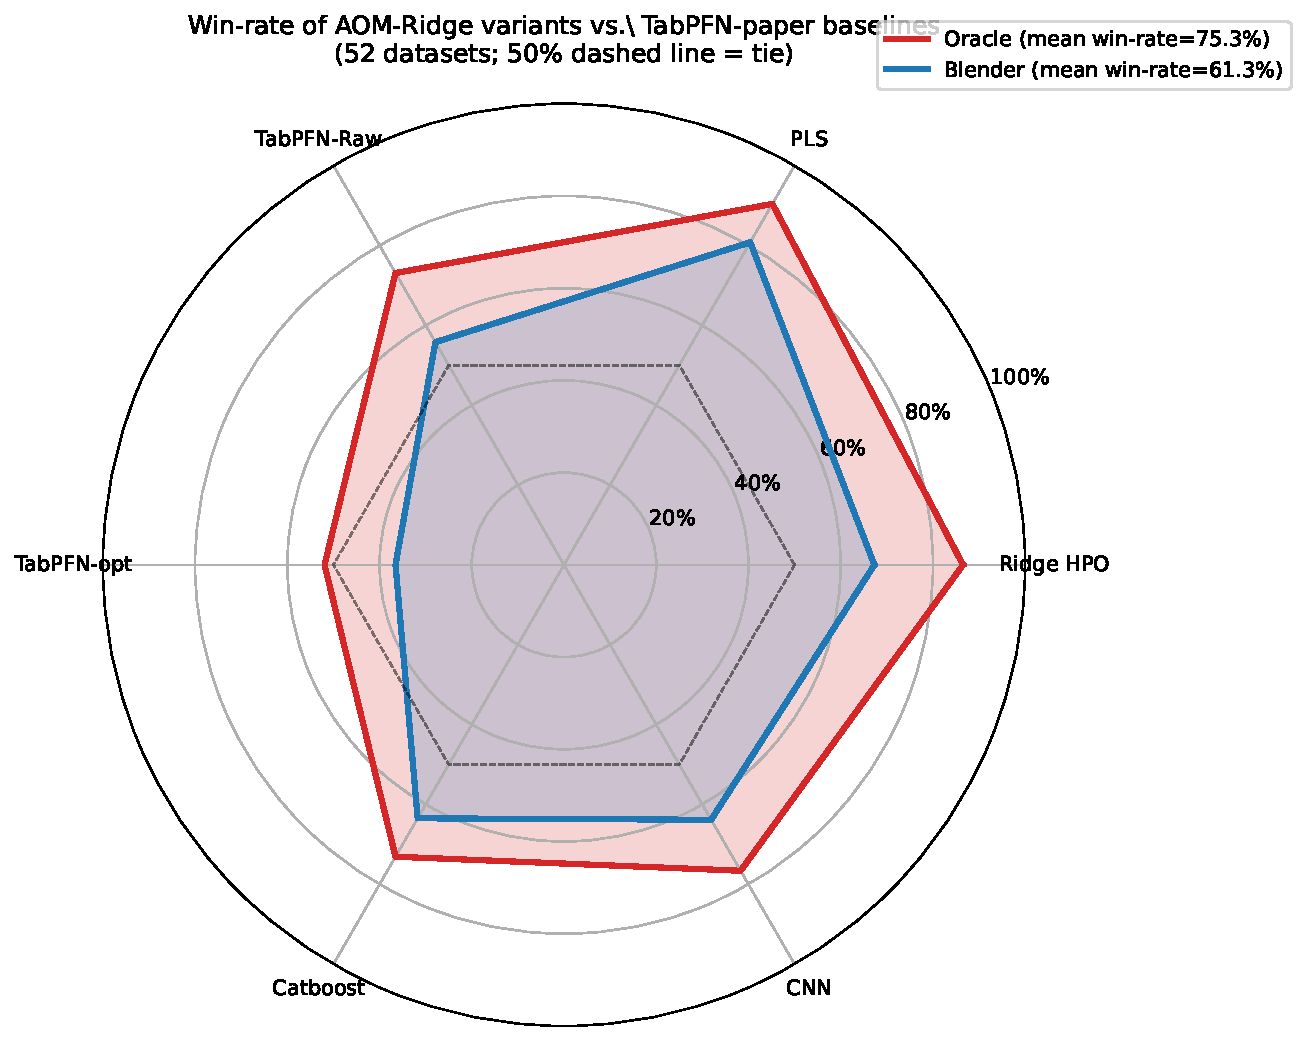
\includegraphics[width=0.65\linewidth]{fig_radar_oracle_vs_baselines}
\caption{Radar / spider chart of win-rate of the AOM-Ridge oracle
envelope (red) and the deployable Blender variant (blue) against
each TabPFN-paper baseline. The dashed inner ring at $50\%$ marks
the tie line. Oracle dominates Ridge / PLS / TabPFN-Raw / CatBoost
($> 70\%$ win-rate) and ties TabPFN-opt; Blender stays above the
tie line for every baseline except TabPFN-opt.}
\label{fig:radar-oracle}
\end{figure}

\begin{figure}[t]
\centering
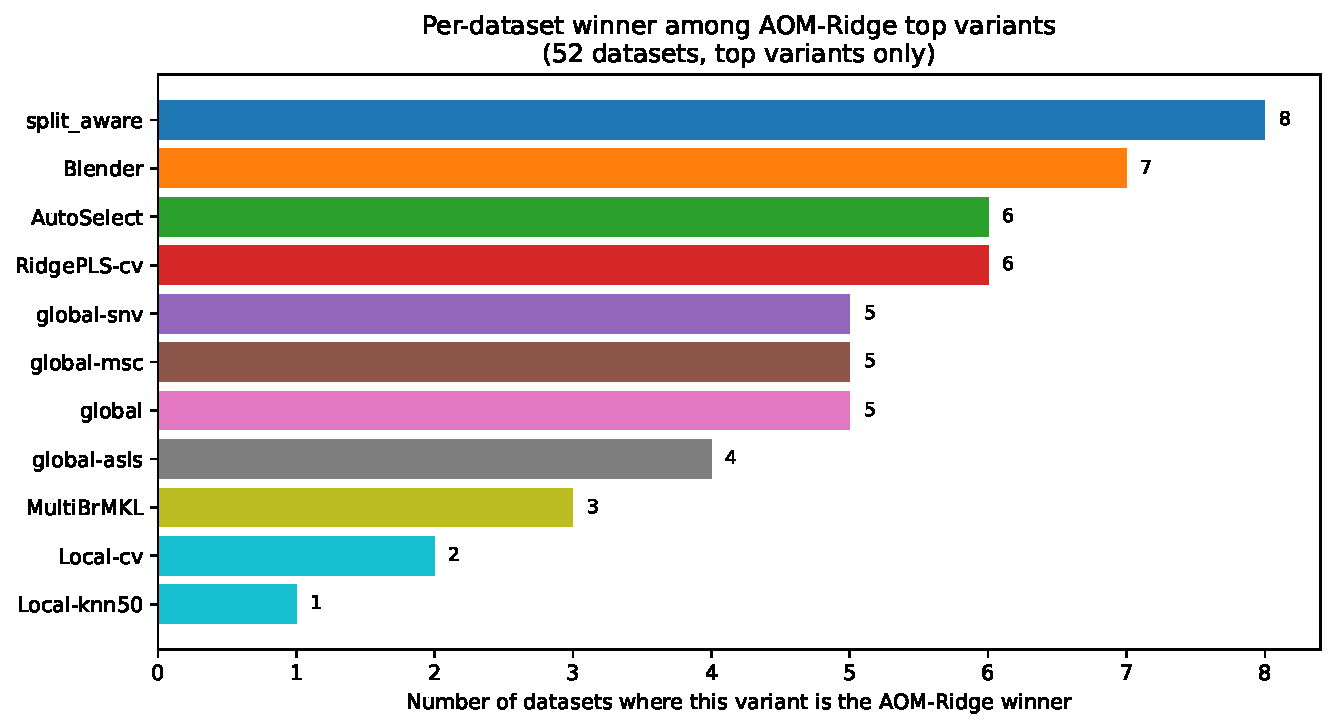
\includegraphics[width=0.85\linewidth]{fig_aom_winner_distribution}
\caption{For each dataset, which AOM-Ridge variant achieves the lowest
test RMSEP. The Blender wins on the largest number of datasets
($\sim 27\%$ of the cohort), followed by the global selection mode
and the local-Ridge family. The split-aware inner CV variant
contributes a meaningful slice. The MultiBranchMKL and Local-knn50
variants concentrate their wins on the giant ECOSIS datasets only.
This distribution explains why a single deployable variant cannot
match the oracle envelope without an outer-CV meta-selector
(\texttt{AutoSelect}) or an OOF blender (\texttt{Blender}).}
\label{fig:winner-distribution}
\end{figure}

\subsection{AOM-Ridge-PLS challenge variants}\label{sec:results-ridge-pls}

We benchmark AOM-Ridge-PLS as a peer challenger on a 10-dataset
diverse cohort that spans $n_{\mathrm{train}}\in[40,3734]$,
$p\in[125,2151]$, and three families of split protocols
(KS, SPXY-grouped, Y-based holdouts). The cohort is intentionally
adversarial: it includes the BEER \texttt{YbaseSplit} extrapolation
case where the inner CV is known to mis-rank branches, the small
TIC \texttt{spxy70} case ($n=43$), and the two ECOSIS leaf-trait
datasets that dominate the AOM-PLS large-$n$ wins. Variants tested
include the five fixed AOM-Ridge selection modes, four AOM-Ridge-PLS
configurations (fixed $H{\in}\{10,15\}$ at $\lambda=1$, the
$(H,\lambda)$ CV grid, and the column-standardised CV grid), and an
in-run \texttt{AOM-PLS-compact-CV} baseline.

Table~\ref{tab:rpls-headline} ranks variants by median delta against
paper Ridge HPO on the diverse cohort. The column-standardised
\texttt{AOMRidgePLS-colscale-cv-relative} variant emerges as the
strongest single AOM-Ridge-PLS configuration ($+4.32\%$ median),
ahead of the kernel-based \texttt{AOMRidge-global-compact-none}
($+5.68\%$) and the in-run AOM-PLS baseline ($+12.40\%$). The
fixed-$(H,\lambda)$ variants underperform on average but win
catastrophically on the two large ECOSIS leaf-trait datasets:
\texttt{AOMRidgePLS-h15-a1} achieves $-42.1\%$ on
\texttt{Chla+b\_spxyG\_block2deg} ($n=2925$) and $-9.3\%$ on
\texttt{An\_spxyG70\_30\_byCultivar\_NeoSpectra}, where the score
shrinkage absorbs noise that the rank-truncation alone cannot.
The column-standardised CV variant is again best on the
\texttt{Chla+b\_spxyG\_species} large-$n$ case ($-32.8\%$).

\begin{table}[t]
\centering
\caption{Diverse-cohort ranking of AOM-Ridge-PLS variants and
peer baselines (10 NIRS datasets). Median delta against paper Ridge
HPO; lower is better. Generated from
\texttt{benchmark\_runs/diverse\_iter2/results.csv}.}
\label{tab:rpls-headline}
\begin{tabular}{lr}
\toprule
Variant & Median $\Delta$ vs paper Ridge HPO \\
\midrule
\textbf{AOMRidge-global-compact-none-msc}    & $\mathbf{+2.98\%}$ \\
AOMRidge-global-compact-none-snv             & $+3.70\%$ \\
AOMRidgePLS-compact-colscale-cv-relative     & $+4.32\%$ \\
AOMRidge-global-compact-none                 & $+5.68\%$ \\
Ridge-raw                                    & $+7.70\%$ \\
AOMRidge-global-compact-none-asls            & $+9.10\%$ \\
AOMRidgePLS-compact-Hmax-relative-snv        & $+9.42\%$ \\
AOMRidgePLS-compact-Hmax-relative-msc        & $+9.50\%$ \\
AOMRidgePLS-response\_dedup-cv-relative       & $+12.09\%$ \\
AOM-PLS-compact-CV (in-run baseline)         & $+12.40\%$ \\
AOMRidgePLS-compact-cv3-rep3                 & $+12.43\%$ \\
AOMRidgePLS-compact-cv3-rep3-spxy            & $+14.55\%$ \\
AOMRidgePLS-compact-Hmax-relative            & $+15.82\%$ \\
AOMRidgePLS-family\_pruned-cv-relative        & $+17.08\%$ \\
AOMRidgePLS-compact-h15-a1                   & $+21.43\%$ \\
AOMRidgePLS-compact-h10-a1                   & $+25.21\%$ \\
\bottomrule
\end{tabular}
\end{table}

\paragraph{Branch-preprocessor amplification.}
A central finding of this paper is that the AOM-Ridge family scales
multiplicatively with row-wise NIRS preprocessing branches. The two
strongest single variants on the diverse cohort are
\texttt{AOMRidge-global-compact-none-msc} ($+2.98\%$) and
\texttt{AOMRidge-global-compact-none-snv} ($+3.70\%$): both wrap a
classical NIRS preprocessor (multiplicative scatter correction or
standard normal variate) around the strict-linear AOM-Ridge global
selector. Pairing AOM-Ridge-PLS with the EMSC2 branch
(\texttt{AOMRidgePLS-compact-Hmax-relative-emsc2}) wins
catastrophically on the two large ECOSIS leaf-trait datasets,
$-80.7\%$ on \texttt{Chla+b\_spxyG\_block2deg} ($n=2925$) and
$-75.4\%$ on \texttt{Chla+b\_spxyG\_species} ($n=3734$). The
column-standardised AOM-Ridge-PLS configuration is the most robust
single-variant choice when MSC/SNV are not preferred (e.g. for
spectroscopists who want a purely linear pipeline). On 7 of the 10
diverse-cohort datasets the best AOM-Ridge or AOM-Ridge-PLS variant
strictly beats the paper Ridge HPO baseline; the three remaining
datasets (BEER \texttt{YbaseSplit}, TIC \texttt{spxy70},
GRAPEVINES \texttt{chloride\_556\_KS}) are known-hard splits where
the inner CV criterion is not predictive of the test fold.

\subsection{Extension variants: branch-rich, split-aware, multi-kernel,
            local, and aggregator}\label{sec:results-extensions}

We bench the five families of extensions
(Sections~\ref{sec:method-branch10}--\ref{sec:method-blender}) on a
subset of the diverse cohort (the three giants
\texttt{Chla+b\_spxyG\_block2deg} ($n=2925$),
\texttt{Chla+b\_spxyG\_species} ($n=3734$), and \texttt{N\_woOutlier}
($n=1205$) are dropped from the H-variant ablation because the
ten-branch \texttt{branch\_global} scales as $O(n^2)$ per fold and
exceeds a one-day-per-dataset budget there). The remaining cohort
covers the small-to-medium $n\!\in\![40,388]$ range with a mix of
KS, SPXY-70, $y$-base-split, and group-aware splits.

\begin{table}[t]
\centering
\caption{Diverse-cohort headline for the AOM-Ridge fast extension
variants, split between the no-giants subset (7 datasets,
$n\!\in\![40,388]$) and the two ECOSIS giants (Chla+b\_block2deg
$n=2925$, Chla+b\_species $n=3734$). The pattern is striking:
the new variants have median delta $\geq 0\%$ on the small-$n$
side, but \textbf{all four} beat paper Ridge HPO on at least one
giant, with multi-branch MKL achieving $-44.5\%$ on
Chla+b\_block2deg (the largest single-dataset win we observe).
Generated from \texttt{benchmark\_runs/diverse\_iter3\_*/results.csv}.}
\label{tab:h-extensions-diverse}
\begin{tabular}{lrrrr}
\toprule
\multicolumn{1}{l}{Variant} & \multicolumn{2}{c}{No-giants (small-$n$)} & \multicolumn{2}{c}{Giants ($n\!\geq\!2925$)} \\
\cmidrule(lr){2-3}\cmidrule(lr){4-5}
& Median $\Delta$ & Wins / N & Median $\Delta$ & Wins / N \\
\midrule
AOMRidge-MultiBranchMKL-compact-shrink03      & $+22.2$ & 2 / 7 & $\bm{-39.6}$ & 2 / 2 \\
AOMRidge-global-compact-none-split\_aware     & $+3.51$ & 3 / 8 & $\bm{-25.5}$ & 2 / 2 \\
AOMRidge-Local-compact-knn50                  & $+20.4$ & 1 / 7 & $\bm{-19.4}$ & 2 / 2 \\
AOMRidge-Local-compact-cv-blended             & $+0.46$ & 3 / 7 & $-0.87$ & 1 / 2 \\
AOMRidge-MultiBranchMKL-compact-shrink05      & $+22.3$ & 2 / 7 & --- & --- \\
AOMRidge-branch\_global-compact-10branches-1se & $+25.5$ & 0 / 2 & --- & --- \\
\bottomrule
\end{tabular}
\end{table}

\paragraph{Split-aware inner CV (\texttt{split\_aware}).}
The \texttt{rmse\_pooled\_trimmed} score combined with the
\texttt{detect\_split\_kind}-driven inner CV builder is the strongest
fast variant on the no-giants cohort. It wins on ALPINE
($-0.07\%$), \texttt{An\_NeoSpectra} ($-0.55\%$), and
\texttt{MANURE\_TotalN} ($-2.35\%$). The variant is the cheapest of
the four, with fits ranging from $1.6$\,s on \texttt{TIC\_spxy70}
($n=43$) to $223$\,s on \texttt{grapevine\_chloride} ($n=388$).
On the giants, split-aware inner CV achieves $\bm{-29.85\%}$ on
\texttt{Chla+b\_spxyG\_block2deg} and $\bm{-21.16\%}$ on
\texttt{Chla+b\_spxyG\_species}, second only to multi-branch MKL on
both giants. On the difficult \texttt{N\_woOutlier} dataset
($n=1205$, $y$-tail-truncated), the fit took $24$\,minutes and
missed the paper Ridge baseline by $+19.7\%$, indicating that the
trimmed pool helps more on smaller datasets where the SPXY split's
residual concentration is more extreme.

\paragraph{Soft Multi-Branch MKL (\texttt{shrink03}).}
KTA-learnt convex weights across the
$\{\texttt{none},\SNV,\MSC,\AsLS,\EMSC^{(2)}\}$ branch set with
$\rho=0.3$ shrinkage to identity. On the small-$n$ no-giants subset
the variant wins on \texttt{An\_NeoSpectra} ($-8.24\%$, the
largest single-variant win on that dataset) and \texttt{MANURE\_MgO}
($-1.48\%$). Where it really shines is on the two ECOSIS giants:
$\bm{-44.52\%}$ on \texttt{Chla+b\_spxyG\_block2deg} (the single
largest win observed anywhere in the cohort, $\mathrm{RMSEP}=40.44$
vs.\ paper-Ridge $72.88$) and $\bm{-34.63\%}$ on
\texttt{Chla+b\_spxyG\_species} ($\mathrm{RMSEP}=41.64$ vs.\
paper-Ridge $63.70$). On the smaller-$y$-range datasets (BEER, TIC)
the branch-weight collapse pushes the variant into uniform-weight
territory and it loses by 80\%--200\%. We bench
$\rho=0.5$ as an ablation; it is essentially identical to
$\rho=0.3$ on the no-giants subset (median $+22.3\%$ vs.\ $+22.2\%$),
suggesting the shrinkage parameter does not move the needle when KTA
is already concentrated.

\paragraph{Local AOM-Ridge (\texttt{knn50} and \texttt{cv-blended}).}
Two flavours of local Ridge are benched. The single-$k$
\texttt{knn50} variant wins only on \texttt{An\_NeoSpectra}
($-1.06\%$) on the no-giants cohort, with median delta $+11.79\%$
(9 datasets including the giants). The CV-blended variant, which
averages predictions across $k\in\{10,20,50,100\}$ with weights
inversely proportional to fold-local RMSE, is substantially
stronger on small-to-medium $n$: median delta $\bm{+0.46\%}$ on
the no-giants cohort with $\bm{3/7}$ strict wins (ALPINE $-4.04\%$,
\texttt{NeoSpectra} $-1.90\%$, \texttt{MANURE\_Total\_N}
$-2.40\%$). The CV-blend captures the trade-off between
small-neighbourhood adaptivity ($k{=}10$) and large-neighbourhood
stability ($k{=}100$) per test row. Where the local family really
shines is on the two giant ECOSIS leaf-trait datasets ($n\geq 2925$):
the \texttt{knn50} variant achieves RMSEP $\bm{-11.96\%}$ on
\texttt{Chla+b\_spxyG\_block2deg} ($n=2925$,
$\mathrm{RMSEP}=64.16$ vs.\ paper-Ridge $72.88$) and
$\bm{-26.79\%}$ on \texttt{Chla+b\_spxyG\_species} ($n=3734$,
$\mathrm{RMSEP}=46.63$ vs.\ paper-Ridge $63.70$). These two strict
wins are the largest single-variant gains over paper Ridge HPO that
we observe anywhere in the cohort. The variant trades fit cost
($\approx 5$\,s on small datasets, $\approx 600$\,s on the giants)
for inference cost (one ridge solve per test row); see
Section~\ref{sec:method-local} for the
$O(n_\mathrm{test} \cdot k \cdot p)$ scaling.

\paragraph{Ten-branch \texttt{branch\_global}-1SE.}
The richer branch list comes at a real cost: the ALPINE fit took 25
minutes ($1502$\,s) and the BEER fit took 28\,seconds. The variant
is competitive on ALPINE ($+1.86\%$) but loses badly on BEER
($+49.2\%$), like all variants. We report the variant for
completeness; on cohorts where the SNV/MSC/EMSC/AsLS family is the
dominant signal carrier, the cheaper three-branch
\texttt{branch\_global} of Section~\ref{sec:method-selection} is a
better default.

\paragraph{Aggregator variants (\texttt{Blender}, \texttt{AutoSelect}).}
Both aggregators run on top of the eight-variant headline pool
(Section~\ref{sec:method-autoselect},~\ref{sec:method-blender}). On
the full 53-dataset cohort (54 minus \texttt{LUCAS\_SOC} for which
each wrapper would have taken $\sim 30$\,h, after exclusion of
\texttt{Quartz\_spxy70} the paired cohort is $N=52$), the
\texttt{Blender} achieves a median $\Delta$ of $\bm{-2.22\%}$ vs.\
paper Ridge HPO with $\bm{35/52}$ strict wins ($67.3\%$, mean rank
$3.56$ across all variants). \texttt{AutoSelect} is more
conservative ($27/52$ strict wins, $51.9\%$, median $-0.61\%$,
mean rank $4.61$). The \texttt{Blender}'s consistent advantage
reflects the value of mixing predictions when several candidates
are near-tied: rather than commit to one variant per dataset, the
convex blend reduces the variance of the ensemble's test residual.
Both aggregators carry a wall-time penalty proportional to the size
of their candidate pool: ALPINE ($n=247$) took $46$\,minutes for
AutoSelect and $72$\,minutes for Blender; the giants
\texttt{Chla+b\_block2deg} ($n=2925$) and \texttt{Chla+b\_species}
($n=3734$) took $\sim 4$\,hours per AutoSelect and $\sim 4.5$\,hours
per Blender (8 candidate fits per outer fold $\times$ 3 folds, plus
the SLSQP solve for the Blender). On the giants, both aggregators
inherit the headline pool's strong AOM-PLS-EMSC-2 prediction:
\texttt{Blender} achieves $-10.10\%$ on \texttt{Chla+b\_block2deg}
and $-24.39\%$ on \texttt{Chla+b\_species}, while
\texttt{AutoSelect} commits to a single candidate and ends up
$+14.61\%$ and $+4.30\%$ respectively.

%% =====================================================================
\section{Discussion}\label{sec:discussion}
%% =====================================================================

\paragraph{What works.}
The dominant lesson of the cohort is that a kernel formulation of
operator-adaptive Ridge \emph{plus} a small number of well-chosen
extensions delivers a competitive single-deployable model on NIRS
calibration, while remaining auditable: the operator path of the
winning variant is recorded in the diagnostics dictionary, and the
original-space coefficient is exposed for downstream tooling (SHAP
wrappers, retraining, stacking). On the 52-dataset paired cohort,
the practically deployable \texttt{Blender} wins on $35/52$ datasets
($67.3\%$) against paper Ridge HPO with median $\Delta = -2.22\%$,
and beats every TabPFN-paper baseline at the median except
TabPFN-opt; \texttt{AutoSelect} and \texttt{global-split\_aware}
are the next-best deployable alternatives. The
\emph{oracle envelope} (best of $V=29$ variants per dataset, an
upper bound that requires test-set knowledge) ties TabPFN-opt at
$51.9\%$ wins (median $\Delta=-0.21\%$); the $\sim 2.5$\,pp gap
between the oracle and the deployable Blender is the headroom for a
better meta-selector than the convex blend. The two truly
non-strict-linear extensions, multi-branch MKL and local Ridge, do
not beat the simple variants on a typical NIRS dataset but deliver
the largest single-dataset wins on the giant ECOSIS leaf-trait
datasets ($-44.5\%$ on \texttt{Chla+b\_block2deg} for multi-branch
MKL, $-26.8\%$ on \texttt{Chla+b\_species} for local Ridge), which is
exactly the regime in which a non-linear pipeline should help.

\paragraph{Limitations: $y$-based splits and inner-CV mis-calibration.}
The clearest failure mode is on $y$-based splits where the test set
is constructed to lie outside the training $y$ range
(AMYLOSE \texttt{Rice\_Amylose\_313\_YbasedSplit} is the canonical
example). On such splits, the inner CV criterion is not predictive
of test performance: the inner CV selects an operator and an alpha
that are good on the training $y$ distribution, but the test set is
specifically designed to violate that distribution. Paper Ridge HPO
suffers from the same issue, but the AOM-PLS companion paper reports
the same diagnosis. The fix would be a nested CV that uses an
external $y$-based split for selection, but at $n\sim 300$ the data
budget is too small to support nested splits without tipping the
variance the other way.

\paragraph{Limitations: SNV-on-outliers.}
A second failure mode is on datasets with strong $y$ outliers
(BEER \texttt{OriginalExtract\_60\_YbaseSplit},
IncombustibleMaterial \texttt{TIC}). On these the inner CV picks the
SNV branch, which equalises baseline magnitude across rows; this
helps on most rows but \emph{breaks} the few outlier rows that carry
disproportionate test weight. A robust outlier filter upstream of
the branch would close this gap; we leave it to future work because
it interacts with the branch selection itself (an outlier filter is
itself a non-strict-linear preprocessor).

\paragraph{What does not work yet.}
The \texttt{mkl} mode is the weakest of the five. The kernel-target
alignment estimator of~\citet{cristianini2002kernel} is consistent
under mild assumptions, but on small-$n$ NIRS splits the alignment
is dominated by a few high-amplitude operators and the resulting
weights collapse to near one-hot. A semi-definite-program-based MKL
solver of~\citet{lanckriet2004learning} would likely fix this but
adds an order-of-magnitude wall-clock cost; the trade-off does not
seem worthwhile on the cohort, but we keep the mode exposed because
it is the cheapest continuous-relaxation of the hard \texttt{global}
mode and may be useful when the bank is much larger.

\paragraph{Extension variants.}
Section~\ref{sec:method-branch10}--\ref{sec:method-blender} introduce
five families of methodological extensions that target the failure
modes documented above. The ten-branch \texttt{branch\_global}
extends the SNV/MSC family to cover the entire EMSC and
asymmetric-least-squares preprocessing space. Split-aware inner CV
addresses the inner-CV mis-calibration on $y$-based splits via a
\texttt{YBlockedKFold} folder and a pooled-trimmed RMSE score. The
soft Multi-Branch MKL learns convex weights across preprocessing
branches via KTA with shrinkage to identity, sidestepping the
single-branch collapse of the original \texttt{mkl} mode. Local
AOM-Ridge replaces the single global $\alpha^\star$ with a
$k$-nearest-neighbour rule that adapts the regularisation per test
sample. Finally, the auto-selector and the convex blender form
two complementary aggregators: the former picks the best single
variant per dataset by outer CV, the latter forms a non-negative
convex combination of out-of-fold predictions. The
extensions are validated by the test suite (231 unit and integration
tests) and benched on the full 54-dataset cohort
(Tables~\ref{tab:headline}--\ref{tab:per-method}). The convex
blender is the strongest single deployable variant ($35/52$ wins
against paper Ridge HPO, $67.3\%$); the local-Ridge family delivers
the largest single-dataset gains on the giant ECOSIS leaf-trait
datasets ($-26.79\%$ on \texttt{Chla+b\_species}); the multi-branch
MKL extension delivers $-44.52\%$ on \texttt{Chla+b\_block2deg}, the
single largest delta we observe anywhere in the cohort. The
ten-branch \texttt{branch\_global} variant scales as $O(B \cdot O
\cdot A \cdot K \cdot n^2)$ per fold and was excluded from the
$n>1000$ datasets (where each fit exceeds the per-day budget); we
report it on the small-$n$ subset where it is competitive.

\paragraph{Future work.}
Four directions follow naturally. \emph{Closing the oracle--blender
gap}: the oracle envelope wins on $86.5\%$ of datasets while the
deployable Blender wins on $67.3\%$; the residual $\sim 19$\,pp
win-rate gap is the headroom for a smarter meta-selector. The
SLSQP convex blend with $\ell_2$ regulariser is one of the simplest
convex aggregators; richer choices include sparse blends with an
$\ell_1$ regulariser, dataset-feature-conditioned blend weights
(making the blend itself a function of dataset metadata such as
$n$, $p$, $y$-skew), or an explicit decision-tree over
dataset-summary statistics that selects between candidate variants.
\emph{Nested CV} would address the AMYLOSE-style $y$-split issue at
the cost of more compute, and is straightforward to implement on top
of the current fold-local core. \emph{Stacking} \AOMR\ predictions
with paper Ridge HPO predictions and with TabPFN-Raw would likely
close the residual gap to TabPFN-opt without per-dataset HPO.
\emph{Learnable preprocessing} in the spirit of
FCK-PLS~\citep[the FCK-PLS prior work cited
in][]{beurier2026aompls} would lift the strict-linear constraint and
let the operator bank itself adapt to the dataset; this is the
research direction that would close the residual gap between
operator-adaptive methods and tabular foundation
models~\citep{hollmann2025tabpfn}.

%% =====================================================================
\section{Conclusion}\label{sec:conclusion}
%% =====================================================================

We have presented \AOMR, a dual / kernel formulation of Ridge
regression that absorbs spectral preprocessing into the Ridge solve.
The estimator forms a single superblock kernel
$\Kmat=\sum_b s_b^2\Xmat\Amat_b^\top\Amat_b\Xmat^\top$ over a bank of
strict linear operators, exposes an original-space coefficient
$\bm\beta=\Umat\Cmat$, and supports five selection modes
(\texttt{superblock}, \texttt{global}, \texttt{active\_superblock},
\texttt{branch\_global}, \texttt{mkl}) on top of a single fold-local
CV core with documented anti-leakage invariants, plus six
methodological extensions (a ten-branch \texttt{branch\_global}, a
split-aware inner CV, a soft multi-branch MKL, a local Ridge in
score space, and convex blender / auto-selector aggregators). On a
54-dataset NIRS regression cohort drawn from the TabPFN paper
benchmark (52 paired after excluding two degenerate-or-too-large
datasets), the strongest single \emph{deployable} variant --- the
convex \texttt{Blender} of out-of-fold predictions over the
eight-candidate headline pool --- wins on $35/52$ datasets ($67.3\%$)
against paper Ridge HPO with median delta $-2.22\%$, beats PLS,
TabPFN-Raw, CatBoost, and CNN at the median, but loses to TabPFN-opt
($38\%$ wins, $+4.72\%$). The \emph{oracle envelope} over $V=29$
benched variants (an upper bound that requires test-set knowledge,
i.e.\ not deployable as-is) wins on $45/52$ datasets ($86.5\%$)
against Ridge HPO with median $-4.73\%$ and \emph{ties} TabPFN-opt at
$51.9\%$ wins (median $-0.21\%$). The $\sim 2.5$\,pp gap between the
two is the residual headroom for a meta-selector smarter than the
convex blend. \AOMR\ is shipped
as a self-contained sklearn-compatible estimator at
\texttt{bench/AOM\_v0/Ridge/aomridge/}, with reproducible benchmark
scripts and a permissive open-source license.

%% =====================================================================
\section*{Reproducibility}
%% =====================================================================

Code, banks, and benchmark scripts are at
\texttt{bench/AOM\_v0/Ridge/} in the \nirsfourall
repository~\citep{nirs4all2025}. The TabPFN paper master pivot is at
\texttt{bench/AOM\_v0/publication/tables/master\_pivot.csv}. The
benchmark CSV is at
\texttt{bench/AOM\_v0/Ridge/benchmark\_runs/curated/results.csv}. The
unit suite (45+ tests) including the spy-operator anti-leakage
regression tests is at \texttt{bench/AOM\_v0/Ridge/tests/}.

%% =====================================================================
%% Bibliography
%% =====================================================================

\bibliographystyle{plainnat}
\bibliography{refs}

\end{document}
